 
%%% The main file. It contains definitions of basic parameters and includes all other parts.

%% Settings for single-side (simplex) printing
% Margins: left 40mm, right 25mm, top and bottom 25mm
% (but beware, LaTeX adds 1in implicitly)
\documentclass[12pt,a4paper]{report}
\setlength\textwidth{145mm}
\setlength\textheight{247mm}
\setlength\oddsidemargin{15mm}
\setlength\evensidemargin{15mm}
\setlength\topmargin{0mm}
\setlength\headsep{0mm}
\setlength\headheight{0mm}
% Recommended layout mentions line spacing 1.5, but this is not relevant to TeX.
% \openright makes the following text appear on a right-hand page
\let\openright=\clearpage

%% Settings for two-sided (duplex) printing
% \documentclass[12pt,a4paper,twoside,openright]{report}
% \setlength\textwidth{145mm}
% \setlength\textheight{247mm}
% \setlength\oddsidemargin{14.2mm}
% \setlength\evensidemargin{0mm}
% \setlength\topmargin{0mm}
% \setlength\headsep{0mm}
% \setlength\headheight{0mm}
% \let\openright=\cleardoublepage

%% Character encoding: usually latin2, cp1250 or utf8:
\usepackage[utf8]{inputenc}

%% Further packages
\usepackage{graphicx}
\usepackage{amsthm}

%% Bibliography
\usepackage{natbib}
\usepackage{url}
\bibliographystyle{unsrt}

%%% Basic information on the thesis

% Thesis title in English (exactly as in the formal assignment)
\def\ThesisTitle{Thesis title}

% Author of the thesis
\def\ThesisAuthor{Name Surname}

% Year when the thesis is submitted
\def\YearSubmitted{1970}

% Name of the department or institute, where the work was officially assigned
% (according to the Organizational Structure of MFF UK in English,
% or a full name of a department outside MFF)
\def\Department{Name of the department}

% Is it a department (katedra), or an institute (ústav)?
\def\DeptType{Department}

% Thesis supervisor: name, surname and titles
\def\Supervisor{Supervisor's Name}

% Supervisor's department (again according to Organizational structure of MFF)
\def\SupervisorsDepartment{department}

% Study programme and specialization
\def\StudyProgramme{study programme}
\def\StudyBranch{study branch}

% An optional dedication: you can thank whomever you wish (your supervisor,
% consultant, a person who lent the software, etc.)
\def\Dedication{%
Dedication.
}

% Abstract (recommended length around 80-200 words; this is not a copy of your thesis assignment!)
\def\Abstract{%
}

% 3 to 5 keywords (recommended), each enclosed in curly braces
\def\Keywords{%
{key} {words}
} 


%% The hyperref package for clickable links in PDF and also for storing
%% metadata to PDF (including the table of contents).
\usepackage[pdftex,unicode]{hyperref}   % Must follow all other packages
\hypersetup{breaklinks=true}
\hypersetup{pdftitle={\ThesisTitle}}
\hypersetup{pdfauthor={\ThesisAuthor}}
\hypersetup{pdfkeywords=\Keywords}

\input title.tex

%%% A page with automatically generated content of the bachelor thesis. For
%%% a mathematical thesis, it is permissible to have a list of tables and abbreviations,
%%% if any, at the beginning of the thesis instead of at its end.

\tableofcontents

%%% Each chapter is kept in a separate file
\chapter*{Introduction}
\addcontentsline{toc}{chapter}{Introduction}
\subsection*{Motivation}

Although the Moore's law\footnote{https://en.wikipedia.org/wiki/Moore's\_law} still applies and the performance of computers is now greater than ever, there still exists some tasks which require a lot of computer power and despite parallelism their accomplishment takes a non-trivial amount of time. Among these tasks are for example computations of some special prime numbers, processing large data sets and many others.

It's natural to ask, how we can speed up such computations. Obvious possibility is to get better hardware, however this is limited by technical progress and can be quite expensive. Widely used approach is to parallelize the computation, that is different parts of the job are run concurrently (in parallel) which results in reduction of the processing time. Generally tasks can be parallelized on different levels. We will talk about parallelism on the level of whole computers, i.e. each computing node is represented by a standalone machine. These nodes are independent and their physical distance can be arbitrary long. The only condition which has to be fulfilled is that the nodes are connected together by the network so they can communicate and exchange data. This approach can be used with big tasks only, because the network communication is relatively very slow and for many tasks it would be a bottleneck. There are also different ways how the general term parallelism can be understood. We will consider so called data parallelism. That is, each computing node runs the same process, only the data differs. This is the main difference from the task parallelism concept in which different nodes can run completely different tasks.

Obviously, not all tasks can be parallelized easily or even are not possible to parallelize at all. On the other hand, there exists also jobs that can be split into smaller parts, each of which can be processed independently and the results then joined together in the end. Concurrent processing of such jobs is quite straightforward and allows use of the data parallelism. These jobs are suitable for our framework.

\subsection*{Goal of the thesis} % (fold)
The main goal is to implement robust framework which is able to split given job, distribute work among participating nodes, which process the assigned parts in parallel, and eventually collect the results and join them together. The domain of suitable jobs is restricted to ones that are described in the preceding paragraph.

The concept of parallelization has been known for many years and many different approaches have been implemented. Some of them are discussed in \hyperref[existing-solutions]{chapter 1}. Nevertheless, the great majority of them uses some kind of hierarchy or at least some control node exists which has different functionality than the others. Main motivation of our work was to provide solution, in which all the nodes are equivalent, each can initiate the process or serve as a computing node. Even in our framework there exists always one node which controls the process while the other ones do the work. But the point is, that every single node can become the initiator (master) or serve as a slave or even both at the same time. Our framework was implemented with the application to the video encoding in mind. However its essence is generic, so it could be easily modified to be used with an arbitrary job which fulfills the above mentioned conditions.

The purpose is to implement framework which conforms to the peer to peer paradigm as much as possible. We also want to keep the logic in the node which have demands to be processed in order to ensure better control and more deterministic behavior. Another important goal is to minimize occurrences of errors in the system and good ability to recover from them. The system is also intended to use personal computers as computing nodes, so the program typically runs alongside other applications.


% section goal_of_the_thesis (end)
\subsection*{Application to the video encoding}
Video files are more or less sequences of images, so called frames. When the file is being played, the images are showed one after the other. They change many times per second so it makes the illusion of smooth video. There are different ways to code the video into the digital form so the need arises to convert the files from one format to other. The program which codes the analog video data to digital or decodes it the other way around is called codec. Some of the well known codecs are for example \textit{H.264}\footnote{https://en.wikipedia.org/wiki/H.264/MPEG-4\_AVC} or \textit{MPEG-2}\footnote{https://en.wikipedia.org/wiki/MPEG-2}. In order to convert the file, each frame has to be re-encoded, which takes quite a big amount of time. This makes the video files ideal for use of our framework.

Before we use it, some more details have to be revealed. Because we usually want to not only watch the video but also listen to some sound, the videos are usually accompanied by one or more audio files and they are packed together in some container. When we want to convert the video, the container has to be opened, the video extracted, processed and stored again. The audio files are not in our concern and we will simply copy them. Common container formats are \textit{avi}\footnote{https://en.wikipedia.org/wiki/Audio\_Video\_Interleave} or \textit{mkv}\footnote{https://en.wikipedia.org/wiki/Matroska}.

There is another important thing. In order to reduce file size and decrease the requirements of rendering the video, the file actually contains only few frames which carry the whole information. These are usually referred to as the key frames. The rest contains only information how the image differs from the previous one. This approach greatly reduces the file size while preserves good ability to recover from errors, e.g. when some part of the file is damaged. Consequence of this fact is, that we cannot split the video file wherever we want, because if the chunk started with some non-key frame, the conversion would not be done properly.

The problematic of video encoding is quite complex and used algorithms are very sophisticated and advanced, so we did not reinvent the wheel and used third party software for the video encoding, namely the ffmpeg and ffprobe from the FFmpeg\footnote{https://www.ffmpeg.org/} project. For the sake of simplicity, the program outputs always video files packed in the Matroska container. The choice of the codec is arbitrary, however it is restricted by the list of options. All of this software is free and published under the GNU General Public License\footnote{https://en.wikipedia.org/wiki/GNU\_General\_Public\_License} or GNU Lesser General Public License\footnote{https://en.wikipedia.org/wiki/GNU\_Lesser\_General\_Public\_License} in case of FFmpeg.

\subsection*{Terminology}
To prevent misunderstandings there is a short list of frequently used terms:
\begin{itemize}
\item \textit{master}(or \textit{initiating node, initiator}) is a node which has work to do, i.e. file to encode. It initiates and controls the process.
\item \textit{task}(\textit{job}) refers to work that should be done, specified by the initiator.
\item \textit{chunk} denotes one part of the split file, which is supposed to be encoded independently.
\item \textit{(computing) node} is one particular entity which communicates with the master and encodes chunks for it. Theoretically, there can be more such entities on one physical computer, because each node is determined by its communicating port and address.
\item \textit{neighbor} is considered every node which is in the database of the node we talk about.
\end{itemize}

\subsection*{Thesis organization}
In the first chapter is given overview of the existing technologies and approaches and our framework is described. Second chapter describes implementation details. Third chapter introduces some experiments and summarizes the results. The fourth chapter is dedicated to alternatives and possible future improvements. In the appendix is then described installation and use of the program.
\chapter{Analysis}\label{analysis}

\section{Known approaches}\label{known-approaches}

The idea of distributed computing has been known since the 70's.
Different approaches have been tried since then. Some of them are
described in this section in order to show different concepts.

\subsection{Client/server architecture}\label{clientserver-architecture}

It's very common example of centralized system. In this pattern is one
central node, known as the server. The rest of nodes, clients, are all
connected to it. All the information is stored at the server. Also all
the important computations happen there. The communication is typically
initialized by the client, which sends a request. The server processes
it and returns the desired result. Pros of this approach are relatively
simple implementation and easy control of the traffic, because all the
data passes through server. Also the data flow can be controlled easily.
However the huge disadvantage is, that the server is by definition a
single point of failure, i.e.~if it goes down, the whole system becomes
unusable. Also, thanks to the asymmetric nature of the system, there
usually has to be more parts of the software, one to run on the server
and the other to run on the clients. The system is dependent on the
server's performance too.

\subsection{Peer to peer
architectures}\label{peer-to-peer-architectures}

\citep{SupPeer} \subsection*{Pure peer to peer network} Peer to peer
paradigm is virtually the opposite of the previous model. Nodes are
completely equivalent to each other. Any of them can join the network at
any time, as well as leave it. This approach means great scalability and
fault tolerance. On the other hand, it requires more complex design and
can encounter problems with security and management of the network. Our
framework implements this model.

\subsection*{Hybrid peer to peer network}

This approach combines the previous two. There exists one node which is
dedicated to serve as a control server. Each node contacts this server
and all the control information pass through it while the data are
exchanged in the same manner as in the pure peer to peer networks. This
approach removes possible problems with the control of the data flow and
provides information coherence while scalability is preserved. However,
the issue with the single point of failure is reintroduced here.

\subsection*{Super peer architecture}

Another try to improve the architecture introduces the concept of the
so-called super peer. It is a computer, usually with slightly better
performance than other nodes, that plays the role of the control server,
but only for a restricted group of nodes. Autonomous groups (clusters)
are thus formed. It has the same advantages as the hybrid network but
the potential super peer failure is not so crucial. Also each super peer
can have backup so the robustness of the network can be very good.

\subsection{Summary}\label{summary}

We showed different implementations of the idea of distributing the
work. Each has its own specifics and may be suitable for some
application. We have chosen to implement our framework to conform to the
pure peer to peer paradigm as much as possible. Although the super peer
architecture offers better control, we decided not to use it for several
reasons. Mainly because our framework is supposed to be used in rather
small networks where this paradigm could be quite exaggerated. Also we
did not use the hybrid network because we definitely want to avoid
presence of the single point of failure.

\section{Existing solutions}\label{existing-solutions}

Since encoding of the video files is quite reasonable task, there was a
few implementations of the similar issue. Some of them served for
academic purposes only, but others found good use case in practice.

\subsection{DVE (Distributed Video
Encoding)}\label{dve-distributed-video-encoding}

D. Hughes and J. Walkerdine from the Lancaster university published in
their paper a solution which is using Lancaster's P2P Application
Framework. They implemented a Java plug-in for this framework which uses
Microsoft Windows Media Encoder
SDK\footnote{https://en.wikipedia.org/wiki/Windows\_Media\_Encoder}.
Their approach was quite similar to ours and they achieved quite
persuasive results. However their solution was usable in the specific
environment only.\citep{DVE}

\subsection{Apache Hadoop}\label{apache-hadoop}

It is sophisticated distributed framework written for the Java platform.
It serves for processing large amount of data and also as a storage. It
provides very good ability to deal with hardware failures. The framework
consists of the HDFS (Hadoop Distributed File System) and the processing
part. The HDFS is a distributed file system which uses
TCP/IP\footnote{https://en.wikipedia.org/wiki/Internet\_protocol\_suite}
sockets for communication between nodes. It uses replication of data to
achieve reliability. It is optimized to store large immutable files
(range of gigabytes or even terabytes). The framework could use
different file system, however, one of its main advantages is the
knowledge about the data locality, hence unnecessary data transfers can
be avoided. This feature may not be available when using some different
file system. The processing part is based on the MapReduce engine, based
on functional programming concept. It basically consists of three steps.

\begin{enumerate}
\item Map - A special function is applied to the local data on each worker node, data are associated with a key. This step can be processed in parallel.
\item Shuffle - The data are redistributed, according to keys. Each worker node obtains data sets with the same key
\item Reduce - The data are processed, in parallel.
\end{enumerate}

A special master node is needed which ensures effective task scheduling.
Generally, the framework is suitable for processing large data sets. It
needs dedicated infrastructure and can achieve very good results. It can
be used in many different applications including image processing,
marketing analysis or data mining. It differs a lot from our solution -
among its complexity and suitability for wide range of tasks, it needs
some nodes with special functionality and also the network of
specialized nodes. In contrast, our solution can operate in almost any
computer network and the computing nodes can serve for other
purposes.\citep{Hadoop} \citep{MapRed}

\subsection{BOINC (Berkeley Open Infrastructure for Network
Computing)}\label{boinc-berkeley-open-infrastructure-for-network-computing}

It is a distributed system, developed on the Berkeley university, which
utilizes computing power of personal computers around the world and
interconnects them in the huge network. It supports multiple operating
systems (the client part). Anyone can voluntarily join the network and
scale it up by granting his computer's performance. After installing the
client application, the system is able to exploit free CPU or GPU
capacity of the computer. The server provides him with a portion of the
given task. After the computation, the results are verified and
uploaded. The system is used mainly for scientific computations. For
example it is used by the well known project SETI@home. The framework is
based on the client-server architecture. The server runs on UNIX
OS\footnote{https://en.wikipedia.org/wiki/Unix}, using common
technologies such as the Apache web server and the MySQL database
server. A PHP language is used.There are also CGI programs and daemons
running on the server. The obvious difference is in use of the
client-server model, nevertheless the philosophy of using regular
computers as the computing nodes corresponds to ours. \cite{BOINC}

\subsection{Gnutella}\label{gnutella}

Gnutella is a peer to peer framework used for file sharing. The nodes
use flood technique with limited number of hops for searching of the
desired data. The positive acknowledgement message is sent when this
data was found, employing the UDP protocol. The file transfer can be
negotiated then. The system is based on the super peer architecture,
which makes it possible to reduce maximum number of hops. Though it is
not used for distributed computation, the data transfers are used which
makes it comparable with our system.\citep{Gnutella}

\subsection{BitTorrent protocol}\label{bittorrent-protocol}

Another interesting file sharing technique is introduced in the
BitTorrent network. The files offered by the node are stored in special
list and a single file download can (and usually do) use more nodes.
This is possible, because the files are divided into pieces and when the
node downloads some piece, it becomes source of this piece for the
others. The pieces are marked so they can be downloaded in random order.
The system provides good redundancy. Another advantage is, that as the
file spreads through the network, the requirements on original
distributor's bandwidth decrease. Eventually the node could not be
needed at all. This protocol is used for file sharing by the BOINC
framework, among many others. It is certainly an interesting alternative
to handle the file transfers. In our framework, the use of this protocol
would not be very convenient and useful, since once the chunk is
processed, it becomes useless.\citep{BitTor}

\section{Framework description}\label{framework-description}

\subsection{Basic overview}\label{basic-overview}

The heart of the program is one executable file, that should be
accompanied by the configuration file. This is discussed in detail in
\hyperref[installation-and-use]{appendix A}. Main options that should be
set are IP address and a number of port which the program should listen
on. It is also essential to provide credentials (i.e.~address and port)
of some node which should be contacted by default. When more nodes are
spawned, the network is formed and the computation may be initialized.
Note that the information about neighbors spread in a nondeterministic
manner, it matters who is contacted by whom. So it's good to have one or
more nodes which are online most of the time and the rest contacts only
these nodes initially. Otherwise the distribution of the neighborhood
knowledge may be quite slow. Once the network is established, the
computation can begin. If one (or more) nodes have tasks to be done, it
can start the process. The file is then processed and divided into
chunks in the initiating node. These chunks are distributed among
neighbors, processed and returned back. Once the initiator has all
chunks back, it joins them together and the process ends.

C++ language has been chosen for the implementation. It allows us to use
standard POSIX socket
\footnote{https://en.wikipedia.org/wiki/Berkeley\_sockets} API
(Application Programming Interface) which is widely used and has been
proven by thousands of applications. Also it provides convenient
functionality thanks to its Standard Template Library while allowing to
use C library functions so it can cooperate well with the OS. Because it
compiles to the native code, it does not need any interpreter, so its
requirements are lower than other languages' such as Java and C\#. This
fact is positive, because it means, that if the application runs in
background and computes nothing, it does not spend many system
resources. The program is supporting Linux operating system, it has been
tested on several Linux distributions. Nevertheless, it conforms to the
POSIX standard
\footnote{https://en.wikipedia.org/wiki/POSIX\#POSIX.1-2001}, so after
some modifications it could be used with any UNIX or UNIX-like operating
system.

\subsection{Neighbor maintaining}\label{neighbor-maintaining}

The diagram which describes the process can be seen in the Figure 1.1.
When the node wants to use other computer's computation capacity, it
naturally has to contact them first. But the node has no prior explicit
knowledge of the network's infrastructure, moreover, this infrastructure
can change dynamically. To solve this, each node maintains the list of
its neighbors. It contains addresses of the nodes which it has contacted
successfully in the past. The list is refreshed periodically, so the
node keeps track of the current network state. Besides this main list
exists another list, which contains potential neighbors. Generally, each
node that has communicated with the given one sometime in the past is
added to the list of potential neighbors. The purpose of this list is to
reduce the amount of time spent with maintaining the neighbors list.
That is, no more than required count of neighbors is maintained, but if
needed, suggestions can be found in this backup list.

Neighbors are uniquely identified by the pair consisting of address and
communicating port. This is sufficient for the potential neighbors,
because before the neighbor is added to the main list, it has to be
contacted. Additional information is then added, so more complex
structure is needed for storing neighbors. This structure contains
information about neighbor's quality, last known state etc. The quality
of the neighbor helps to prefer one neighbor to another while picking
the one to contact. It is updated after each chunk is delivered from the
given neighbor and reflects the neighbors computation power together
with the speed of the connection.

\subsection*{Initialization and discovery}

This may be the most important part of the process. Its overview is
given in Figure 1.1. The node is provided with the address and port of
the neighbor which should be contacted by default, that is, when the
neighbors list is empty. Each node has minimum count of neighbors which
should be in its list. This number is checked periodically. In case that
the count of confirmed neighbors is too small, the list of potential
neighbors is checked. If it's empty, the node has to obtain more
neighbors so it picks one of its neighbors, contacts it and receives
some suggestions. If it has no neighbors, the default node is contacted.
Once the suggestions are received, the node adds the new addresses to
the list of potential neighbors. When the list contains some potential
neighbors, the node can contact them, confirm, and add as regular
neighbors.

\begin{figure}[h]
\begin{center}
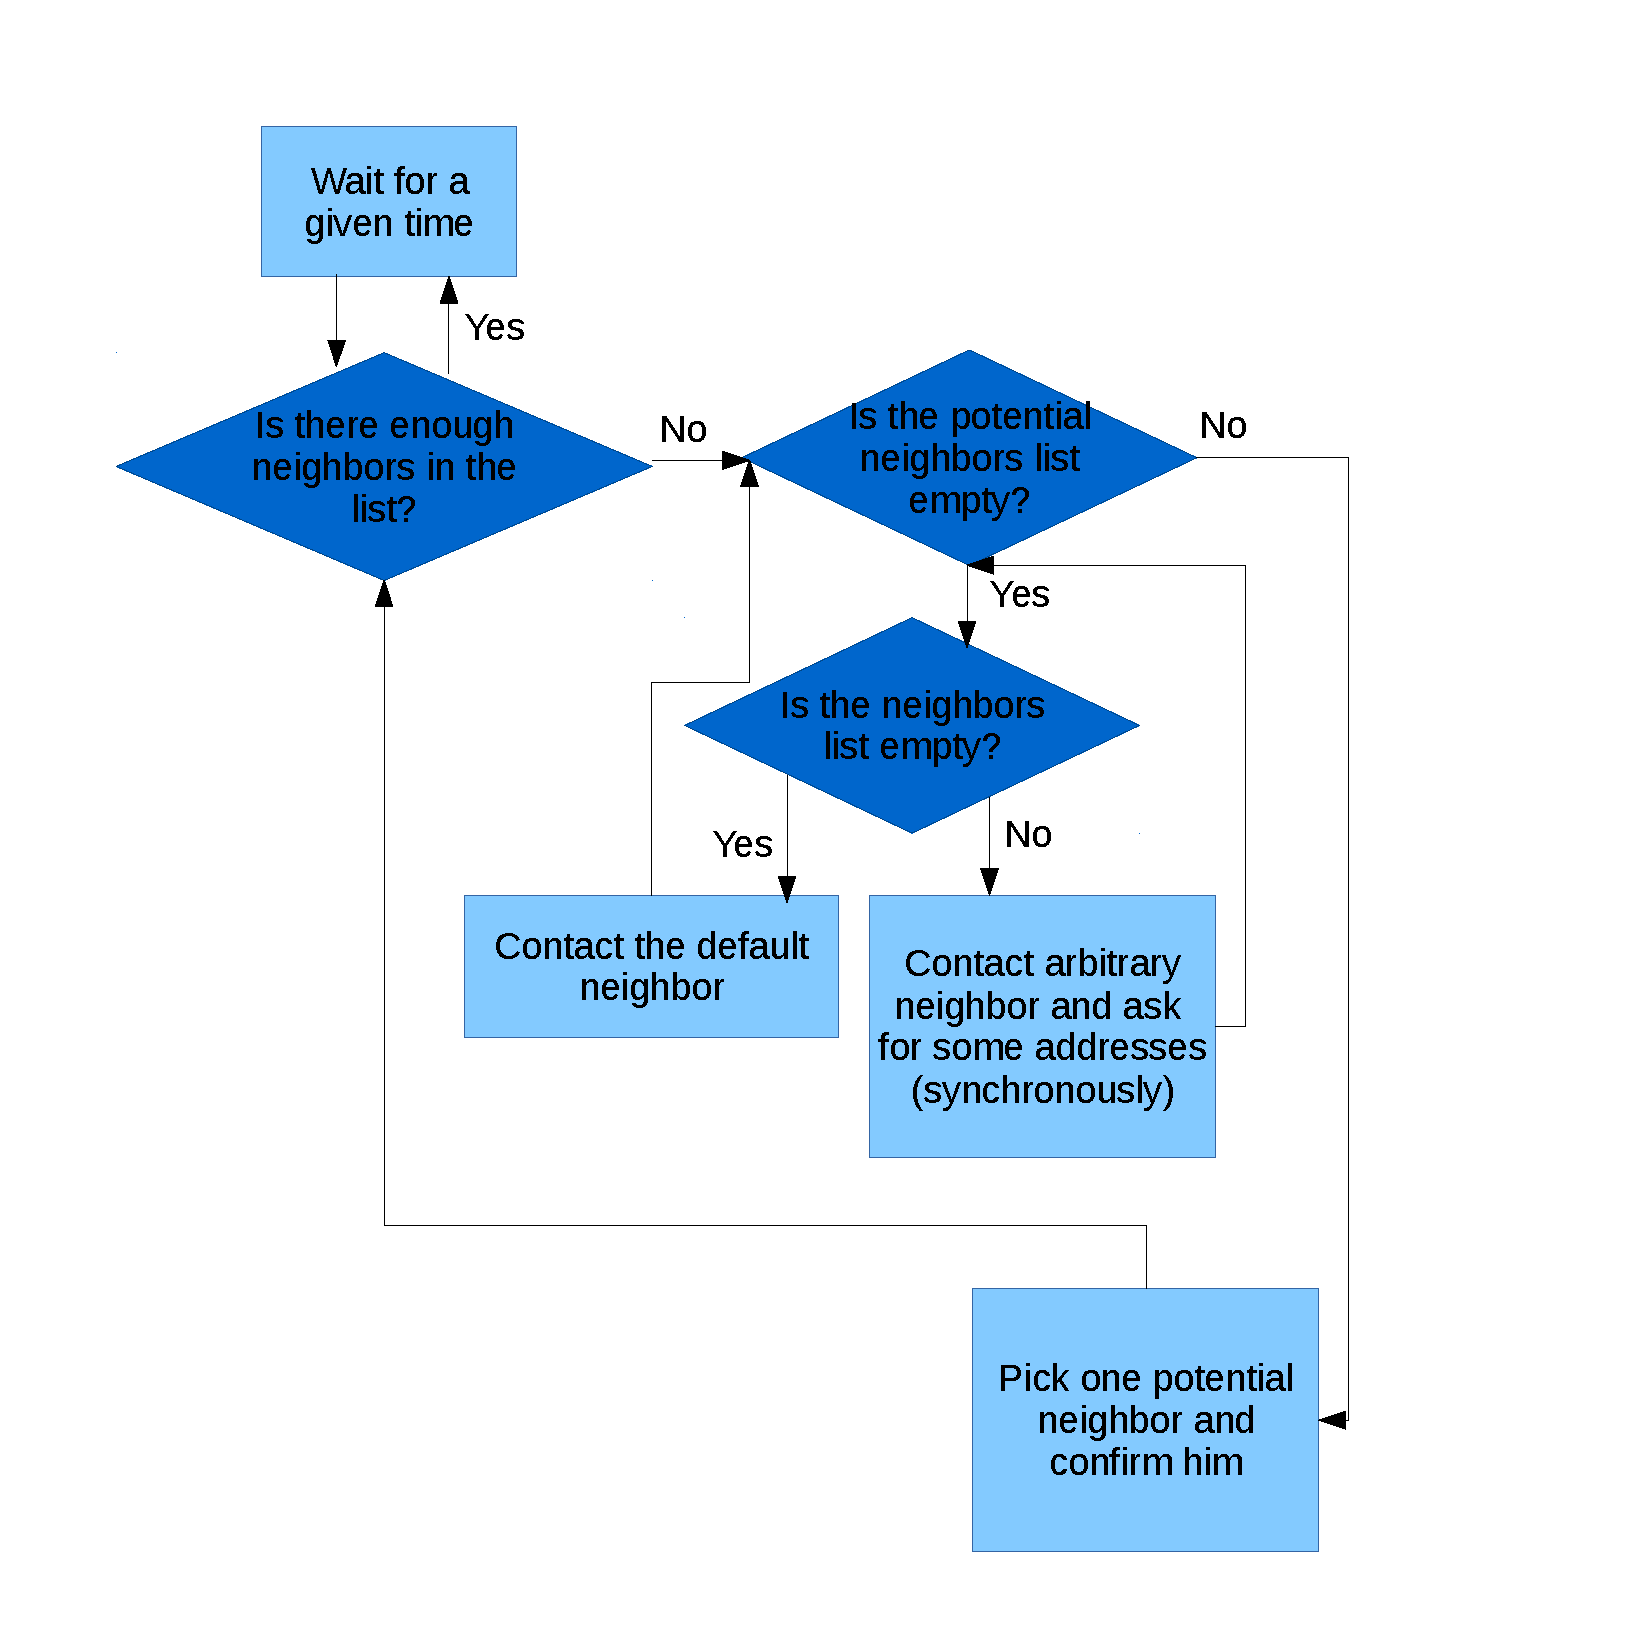
\includegraphics[scale=0.40]{./img/workflow_neighbors.pdf}
\caption{Maintaining the neighbors}
\end{center}
\end{figure}

\subsection*{Gathering neighbors}

When the initiating node has not enough neighbors and it needs more
neighbors with free computation power, it can use another mechanism to
collect them. This mechanism uses a flood technique to spread the
request among the nodes in the network. The request is send to each
neighbor, which spreads it further in the same manner. However, the
request is equipped with time to live value that is decreased after each
hop. Because of this, it does not spread forever nor too far. Once the
node receives a request and is not busy, it contacts the initiator
directly. It can then add him to the list of potential neighbors and
later possibly as the regular neighbor.

\subsection*{Withdrawing from the network}

When the node wants to leave the network it has to abort the process, if
it is the initiator. Then a special message is sent to each neighbor,
which informs them so they can react accordingly. That is, if the
neighbor has tasks to be processed for the leaving one, it removes them
from the queue and then removes the neighbor itself. Removed neighbors
are completely lost, they are no longer stored in either of the lists.
The process of saying goodbye to neighbors is asynchronous, the
withdrawing node does not wait for any confirmation. There are several
reasons for this behavior. Waiting for the response could cause a
deadlock under some specific circumstances, e.g.~if the contacted
neighbor went down unexpectedly. Also, there is no need for it, since
there is no possibility to stop the node from withdrawing.

\subsection*{Neighbor's failure}

There is no guarantee that all the neighbors leave the network properly.
The program itself can encounter error or be terminated violently.
Another possibility is some unpredictable error of physical character,
for example power failure, network problem etc. In those cases it's
essential for the other nodes in the network to be informed about this
fact. Especially it's very important for the initiator who had some
tasks processed by this node. In order to ensure handling of this
possibility, the neighbors list is checked periodically. If some
neighbor does not respond, it is removed from the list and all the data
connected with it are treated accordingly. Namely the chunks assigned to
it are resent.

\subsection{Distribution of chunks}\label{distribution-of-chunks}

Once the file is split, the chunks has to be distributed, processed and
finally collected. To achieve this, we must deal with several issues,
which are described further.

\subsection*{Life cycle of the chunk}

Its description is displayed in the Figure 1.2. Firstly, we have to keep
track of every chunk's state. That is, we have to know whether the chunk
is waiting in the queue, has been sent to be processed or has returned
already. Each chunk is represented by the dedicated structure, which
holds information about it. It also carry information essential for the
transfer. This structure is further described in
\hyperref[implementation]{chapter 2}. From now on we will use the term
chunk for both the physical file and the reference.

Typical chunk's life cycle looks like this: The chunk is created and
pushed to the waiting queue. Later it's popped out and transfered to the
processing node. There it is enqueued for processing, then processed and
sent back. Meanwhile the initiator holds the reference in the list of
tasks being processed. In case of failure of the processing node, the
chunk is pushed to the waiting queue again. Also when the chunk waits
for return, it's checked periodically and if the computation takes too
long, it's resent too. This happens because the respective chunk's
encoding could fail or there were some problems with it. There is a
possibility, that it will be computed sooner by another neighbor. Note
that this can cause the situation, when one task is being processed by
more than one node. However it's not a problem at all, because if the
chunk returns more than once, it simply is not accepted. Furthermore,
when the chunk returns, all neighbors that have it assigned are
notified, so this situation should not happen at all. Once the chunk
returns successfully, the reference is moved to another list, where it
waits for completion of the task. When all the chunks are collected, the
joining process may begin and the task execution ends.

\begin{figure}[h]
\begin{center}
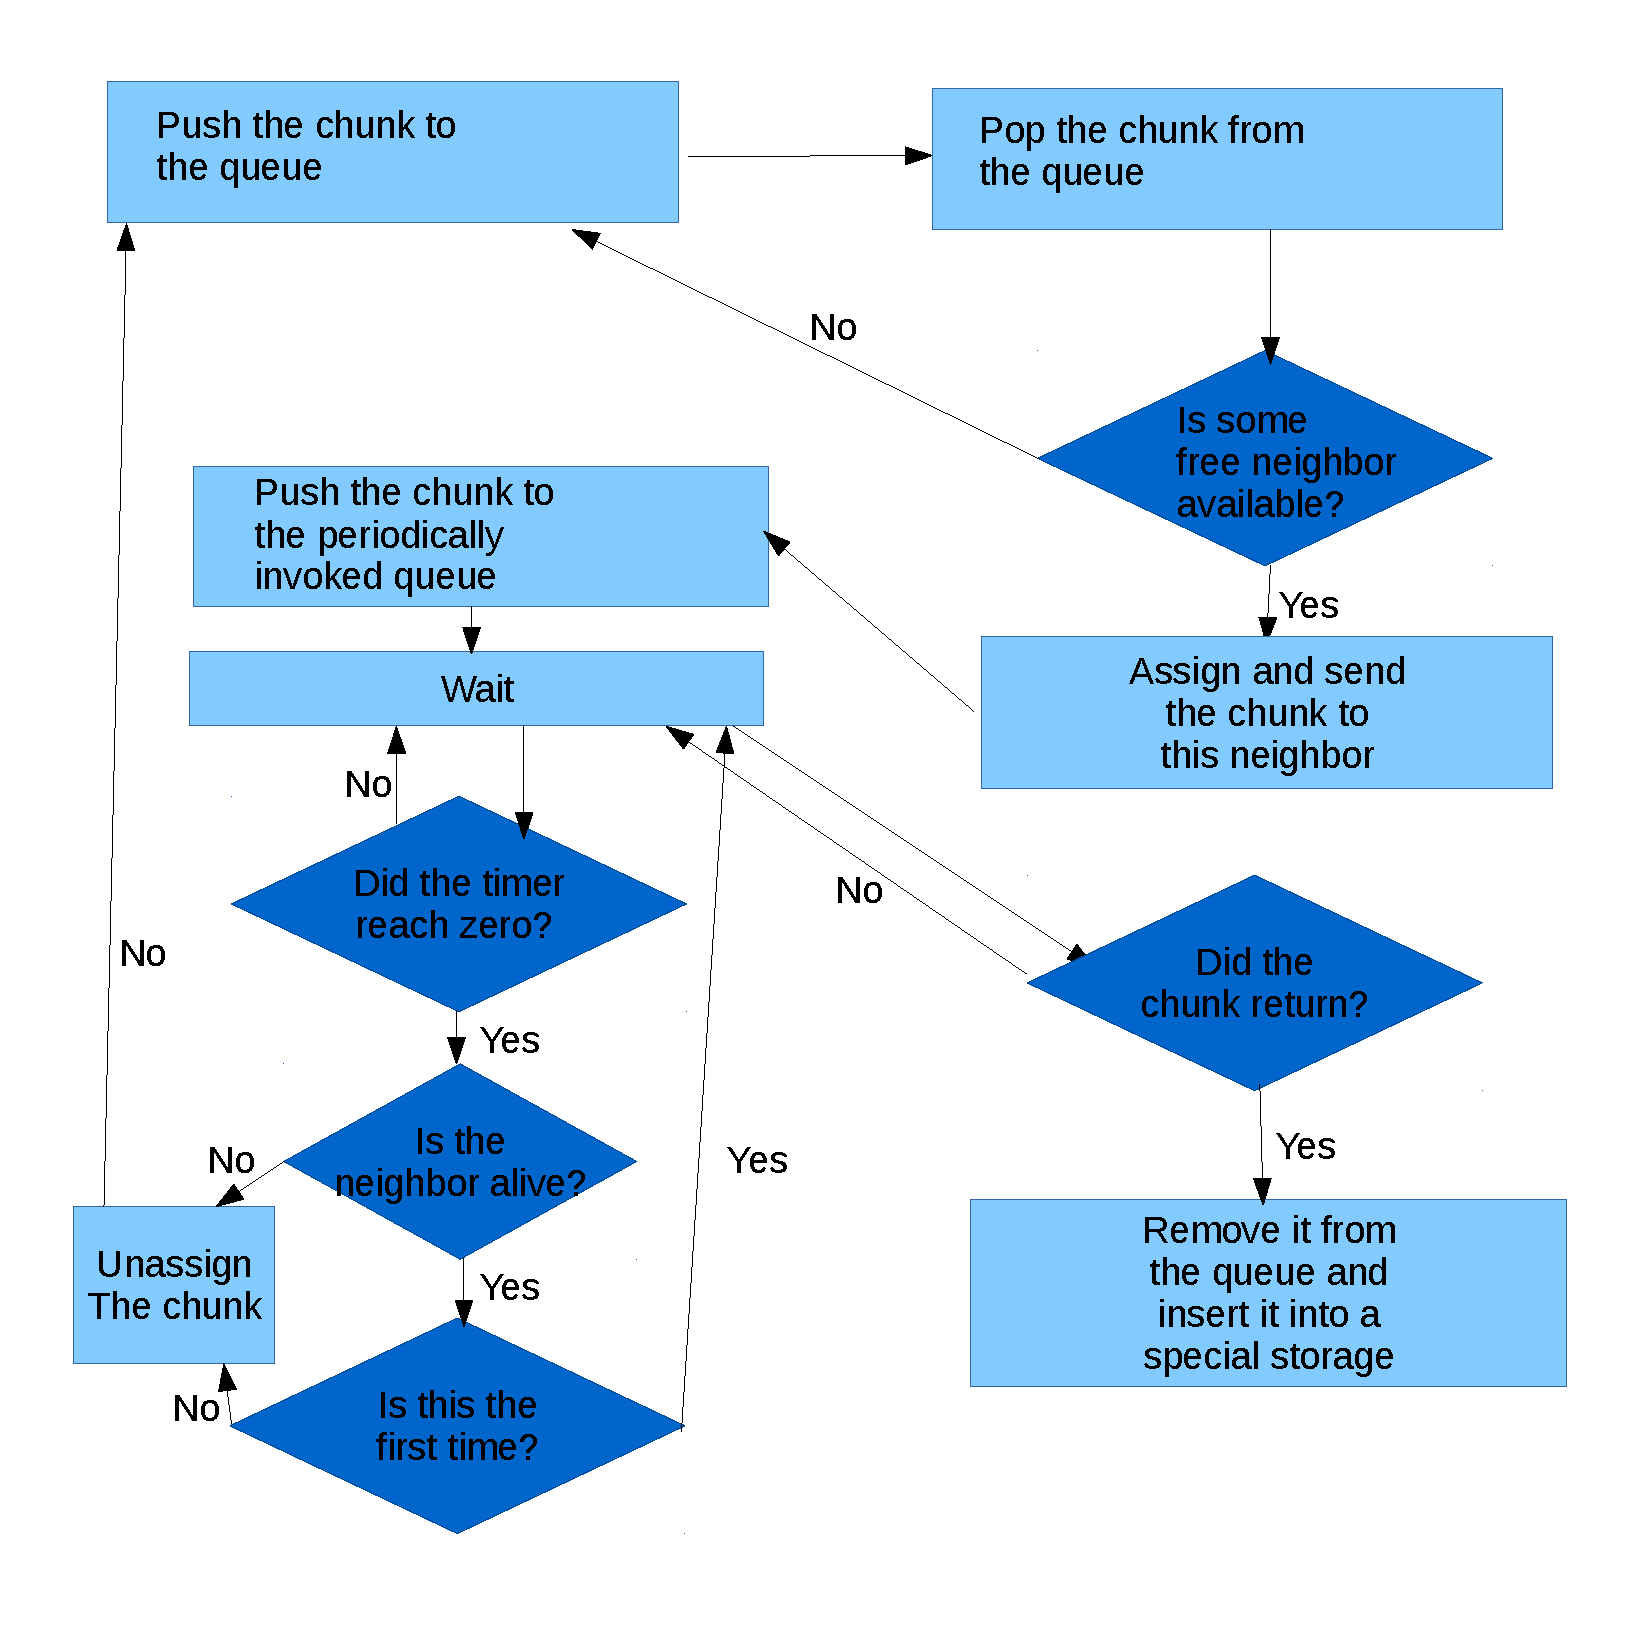
\includegraphics[scale=0.40]{./img/workflow_chunks.pdf}
\caption{Processing a chunk - initiator part}
\end{center}
\end{figure}

\subsection*{Storing files}

Tightly coupled with this process is the problem of storing the files.
Four files have to be created during the processing of every chunk. The
first one is created when the original file is split. This file can't be
removed until the processed chunk returns, because it has to be
available in case that the conversion fails for some reason. Another two
files are created at the processing node, one for the input and one to
store the output. The last file is created at the initiating node again
to hold the processed chunk. This means, that the initiator has to have
free disk space at least twice larger than the resulting file.

\subsection*{Picking neighbors}

Last but not least we have to choose policy to whom the chunks are
distributed. We want to achieve as big speedup as possible, while
preserving rather small list of neighbors. When the chunk is popped out
from the queue, the initiator looks for suitable neighbor. That is the
neighbor which has free status in the corresponding structure. If no
such neighbor is found, the chunk is re-queued and another try is
postponed. Also the gathering process described in the previous section
begins. If some neighbor is available, the chunk is assigned to it and
the transfer may begin. The initiator keeps track how many chunks were
sent to the particular neighbor and it does not send more than specified
count to one neighbor because it could potentially cause delay. The flag
indicating whether the neighbor is free helps to control the flow. Each
time chunk is assigned to the neighbor, the flag is set to false value
to prevent sending more chunks in parallel. It's set to true again after
the successful completion of the transfer. When the neighbor is too
busy, it can express it in the communication, so the flag is set to
false to prevent overloading of the neighbor. The flag is also refreshed
during every periodic check.

\subsection{Security issues}\label{security-issues}

The present implementation is possibly vulnerable to some security
threat. This is caused partly by the pure peer to peer nature, because
it is difficult to control the traffic and authorize all nodes in
dynamic environments like this. It also was not our aim to solve this
issue. The framework is supposed to be used mostly in LANs (Local Area
Network) where all the peers are trustworthy. Otherwise it could be
compromised easily. For example when the encoded chunk arrives, it is
not checked whether it has been sent to this node or not. So a malicious
chunk could be infiltrated causing bad output or even failure of the
joining process.

\subsection{Networking handling}\label{networking-handling}

The network communication is the most important part of the framework.
Standard C library functions and structures were used which are
conforming to
POSIX.1-2001\footnote{https://en.wikipedia.org/wiki/POSIX\#POSIX.1-2001}
standard. Although the program is intended to be used on the
UNIX\footnote{https://en.wikipedia.org/wiki/Unix} or UNIX-like operating
systems, it should be portable to the Microsoft Windows systems as well
thanks to the use of this standard. To preserve simplicity, all the
network communication makes use of the TCP (Transmission Control
Protocol)
\footnote{https://en.wikipedia.org/wiki/Transmission\_Control\_Protocol}.
The system primarily uses the IPv6
\footnote{https://en.wikipedia.org/wiki/Internet\_Protocol} addresses,
but it can be run in the mode which uses addresses of the IPv4 family
only. Additional and more detailed information can be found in
\hyperref[implementation]{chapter 2}.

\subsection{User interface}\label{user-interface}

To provide interaction with the user, the
curses\footnote{https://en.wikipedia.org/wiki/Curses\_(programming\_library)}
library is used. This library makes it possible to control the terminal
screen. That means, the application does not require any special GUI
(Graphical User Interface) libraries and is able to run interactively
even on machines without the X server. The control is rather simple,
offering possibilities to load the file, start or abort the process,
show information about neighbors and so on. The interaction require only
a keyboard, no mouse is needed at all. Concrete information together
with some examples can be found in
\hyperref[installation-and-use]{appendix A}. Detailed information about
the implementation, namely the synchronization problems are discussed in
\hyperref[implementation]{chapter 2}.
\chapter{Implementation}\label{implementation}

This chapter describes some of the used mechanisms in more detail. It
also introduces some classes and methods, but it is not supposed to
serve as a detailed and full documentation. The
Doxygen\footnote{https://en.wikipedia.org/wiki/Doxygen} software has
been used to generate documentation so the complete overview of the code
can be found in the attached
HTML\footnote{https://en.wikipedia.org/wiki/HTML} documents. The program
is implemented in the C++ language. This allows us to use the standard C
library functions. Also the functionality provided by the C++
STL\footnote{https://en.wikipedia.org/wiki/Standard\_Template\_Library}
is exploited. Some of its containers are used as a base for containers
with synchronized access implemented in the framework. Some of the
functionality from the C++11\footnote{https://en.wikipedia.org/wiki/C++}
standard is also used, so the use of the program is limited to computers
with compiler supporting this standard.

\section{Networking}\label{networking}

One of the most important issue is how to handle the networking. The
chosen approach will be described in this section. As it has been said
already, the program uses TCP for network communication. This is
certainly good option when we want to handle data transfers, however, it
can be considered unnecessarily demanding for simple tasks. To preserve
the implementation simple, we chose not to use UDP. To utilize the
possibilities of the operating system, standard socket API is used.
Information about addresses are stored in the \textit{sockaddr\_storage}
structures which are suitable for storing both IPv4 and IPv6 addresses.
There are also some helper functions to work with address structures
which are generic in the use of an address family. To provide easy
manipulation with addresses, the structure \textit{MyAddr} was created
which groups the related functionality together. This approach makes it
possible to switch between both IP versions easily.

\subsection{Spawning connections}\label{spawning-connections}

The ultimate class to handle the connections is the
\textit{NetworkHandler} class. It provides all the necessary
functionality. Each instance of the program binds to the given listening
port and starts accepting connections. When the connection is accepted,
new thread is spawned to handle the connection. When the program wants
to make the connection, it provides structure referring to a given
neighbor together with the commands to be executed to the
\textit{NetworkHandler} instance. The connection is then spawned and
handled.

Here we encounter the topic of commands. Each action is represented by a
set of commands that implements it. Commands are instances of a class
which inherits the class \textit{Commnand}. Each command consists of two
parts. When one node initiates the connection, it provides the vector of
commands to be executed. They are processed in the loop in the following
manner: The command's \textit{execute} method is invoked. It
communicates over the network. First it sends name of the command to be
invoked in the peer node. The peer's thread loops too. First it reads
the name of the command and then it invokes it. In that moment there are
command methods running in both nodes and they can communicate. When
they end, the receiving node waits for another action. Meanwhile the
initiating node spawns next command from the vector. If the vector is
empty, the initiator ends the connection. This mechanism is used to
handle all the network communication. What happens in case of problems
is described in the section about handling errors.

Incoming connections are always handled asynchronously. Nevertheless,
the outgoing connections may be handled in the synchronous way. It can
be essential sometimes. For example if the node needs to obtain some
potential neighbors because his list is empty, it has to wait until the
action ends, because if it just sent the request and continued, it would
probably find the list still empty.

\subsection{Protocol}\label{protocol}

As it was said, the communication uses commands. Thread that handles the
incoming connection is provided with respective file descriptor and
address of the communicating node. First data that appears are
considered as the listening port number of the node, so it can be
identified in the neighbors list or added to the list of potential
neighbors. Then the name of the command is sent, which is represented by
the \textit{enum} type. If no error occurs, the confirmation is send and
the appropriate command's method is invoked. After returning from the
method, another command is read. If there are no data left, the
connection is closed. The most important commands are listed below.

\begin{enumerate}
\item {\large Commands for maintaining}
\begin{itemize}
\item  \textbf{Confirm} - Confirms the potential neighbor, adds the node to the neighbors list.
\item  \textbf{Ask} - Asks the neighbor for the list of addresses, receives the list and adds the addresses to the potential neighbors list.
\item  \textbf{Ping} - Verifies that the neighbor is alive, refreshes its status.
\item  \textbf{Cancel} - Cancels the request for particular chunk's encoding.
\item  \textbf{Goodbye} - Notifies the neighbor that the node itself is withdrawing from the network.
\end{itemize}
\item {\large Commands regarding transfers}
\begin{itemize}
\item  \textbf{Distribute} - Sends both the reference and the chunk itself during distribution.
\item  \textbf{Return} - Returns the encoded chunk back, together with the referencing structure, which is updated with the data about encoding and transfers.
\item  \textbf{Gather} - Spreads the request of the initiator to obtain more neighbors.
\end{itemize}
\end{enumerate}

\subsection{Transferring the data}\label{transferring-the-data}

First problem every network application has to deal with considers the
byte order. The POSIX sockets API provides set of functions to deal with
it. Namely it's \textit{htons} and \textit{ntohs}, or \textit{htonl} and
\textit{ntohl} respectively. These functions convert the native
representation of short (long) data types to the network byte order. The
framework uses these function.

\subsection*{Basic transfer functions}

Each of the functions mentioned in this paragraph has basically two
parts. One for sending and its receiving counterpart. Integers are
stored as the \textit{int64\_t} type which ensures correct communication
even between 32 and 64 bit nodes. They are sent using the mentioned
converting functions. When the string is transfered, first is sent the
length of the string, followed by the appropriate number of characters.
Commands are sent as numbers, wrapper functions are used which converts
between the \textit{enum} type and \textit{int32\_t} explicitly. Sending
the structures containing the addresses is managed by another special
function. It converts the address to string and sends it in this form,
followed by the port number. This allows to handle both IPv4 and IPv6
addresses, the format is recognized during the reversed conversion.

\subsection*{Transfering files}

The most delicate network task is to transfer the files. The file is
first check, and its size is determined. Then it is sent and then the
function repeatedly reads part of the file to buffer and sends it until
whole file is processed. The count of sent bytes is compared with the
actual file size in the end. The receiving side accepts the bytes and
writes it to the file continuously, the file size is checked in the end.
The data are first written to a temporary file which is renamed after
the successful transfer. This mechanism prevents inconsistency of the
received files. Each file is referenced by the
\hyperref[the-transferinfo-structure]{structure}. Among other things
this structure stores counter of unsuccessful sent tries. If the counter
exceeds given limit, the neighbor is treated as invalid and his state is
set to non-free. The file is also checked, if it is not valid for some
reason (the splitting process has encountered some error), the whole
process has to be aborted because there is no way how to fix one
specific chunk file.

\subsection{Handling errors}\label{handling-errors}

Unfortunately the network environment is quite error prone and all the
action has uncertain results. Moreover, the communication can be
interrupted at any time. Because of this it is important for the network
application to be able to deal with different error situations.

\subsection*{Errors during the connection handling}

Almost all the functions indicates error state by the negative return
code. These codes are checked so the error can propagate. If some error
happens during the control communication, the loop that handles the
connection simply brakes, so the connection is closed. The commands are
invoked in the try-catch block, so if the data have been corrupted or
the synchronization has been lost, the next invalid command name raises
an exception and the error is handled. The loss of synchronization may
be detected thanks to the obligatory confirmation of every command.

\subsection*{Other errors}

If an error happens during the file transfer, the receiving side detects
inconsistency thanks to checking of the file size, so the bad file can
be removed. Generally, if any error is encountered during the
communication, the corresponding execute method indicates it by its
return value, so it can be propagated further. The signal handler also
has to be set to cover situations when the connection is destroyed
unexpectedly and the
SIGPIPE\footnote{https://en.wikipedia.org/wiki/Unix\_signal} is
delivered.

\section{Structures' overview}\label{structures-overview}

This section describes two main structures that are used in the
framework. They common sign is, that they inherit from the
\textit{Listener} class, so they have to implement the invoke method.
This fact makes it possible to use them as
\hyperref[periodic-actions]{periodic listeners}.

\subsection{The TransferInfo
structure}\label{the-transferinfo-structure}

This structure serves for referencing the chunk. It contains flags used
for transfer, addresses (source and destination), information about the
video and path locating the physical position of the file. This field is
important because it makes it possible to reference the file. It is
changed several time during the process; as the state of the chunk
changes, it it located in various directories and it is important to
keep the value of the field actual. The structure also contains
information which help to determine the encoding process and some
statistics which describes the result. These are used to compute and
update the quality of the neighbor. The structure is also equipped with
a pair of methods that make it able to transfer it over the network.
This simplifies the usage of the structure. When the referenced chunk is
waiting for return, the corresponding method is invoked periodically. It
decreases the timer. For the first time the timer reaches zero the
neighbor which has this chunk assigned is checked. If it is alive, the
timer is set one more time. If the neighbor doesn't respond or the timer
reaches zero for the second time, the chunk is resent.

\subsection{The NeighborInfo
structure}\label{the-neighborinfo-structure}

Instances of this structure are kept in the
\hyperref[neighborstorage]{NeighborStorage class}. They represent the
neighbor, that is its address and listening port. It also keeps the
information about quality of the neighbor. The time elapsed from the
last check is stored too. Periodic invocation causes the timer to
decrease and possibly contact the neighbor to refresh the state.

\section{Important classes}\label{important-classes}

\subsection{The NeighborStorage class}\label{the-neighborstorage-class}

It is used for storing the \textit{NeighborInfo} structures. It provides
several methods to maintain neighbors list while preserving
synchronization. This is crucial, because the information about neighbor
can change any time but it's desirable to keep our knowledge consistent.
The class exists in one instance and helps to keep the information about
neighbors in one place, so the manipulation can be controlled.

\subsection{The NetworkHandler class}\label{the-networkhandler-class}

This class is used to handle all the networking issues. It provides
functionality to spawn the connections or contact neighbors. It also
holds the list of potential neighbors. This list differs from the
neighbors list, because besides address and port, which are necessary,
no further info is stored about potential neighbors. Also, most of the
other classes have not got a notion about this list. When the lack of
neighbors appears, simply the function \textit{obtainNeighbors} is
invoked, which uses the list internally. This class also handles adding
of the new neighbors.

\subsection{The Data class}\label{the-data-class}

It is a singleton class which helps to keep all the data at one place.
It also makes the data accessible from anywhere in the program. It holds
the instances of the \textit{NeighborStorage}, \textit{State} and all
the \hyperref[queues]{queues} that are used during the transfer and the
encoding process.

There are more significant classes such as TaskHandler and
WindowPrinter, which will be discussed in the corresponding sections.

\section{Periodic actions}\label{periodic-actions}

The framework uses a mechanism which invokes some actions periodically.
Pros and cons of this approach are described in the respective sections,
namely
\hyperref[problems-alternatives-and-possible-improvements]{the alternatives}.
To implement this mechanism, separate thread runs that loops and once
after each time quantum it invokes methods of structures that inherit
from the \textit{Listener} abstract class and are stored in the special
queue. The time quantum is defined as a constant, so all timers actually
express count of the quanta left. Obvious disadvantage of this approach
is busy waiting that is used in the loop. Alternative approach could use
a signal handler and setting an alarm. However, this could lead to not
necessary asynchronous interrupts. Since the mutexes are used to avoid
race conditions, a problem could occur if the signal interrupted some
method holding a ``bad'' mutex.

\section{Queues}\label{queues}

As it is described in the corresponding
\hyperref[distribution-of-chunks]{section}, the references to chunks can
appear in different queues. The chunk's placement depends on the state
in which it is. Since the whole process is nondeterministic, different
conditions may occur and more than one thread could need to work with
the queue at one moment. This means, that some way of serialization has
to be provided. Because of this, the
\textit{SynchronizedQueue structure} has been created. Basically it
provides usual functionality that could be requested from the queue, but
ensures handling race conditions because only one thread at a time can
access the underlying data. This is ensured by the \textit{mutex}. The
\textit{pop} method also uses the conditional variable, so if there are
no data that can be popped at the moment of invocation, it blocks and
waits for a signal.

\section{Working with input and
output}\label{working-with-input-and-output}

All the file operations are customized for use on the UNIX operating
system. Nevertheless, there is possibility to implement respective
functions to work on different operating systems easily.

\subsection*{File operations}

Each chunk is stored in a separate file. For this reason several
functions were implemented to allow easier work with the file system.
These include functions for manipulation with the filenames, controlling
files and working with directories. Also there is a generic function
which spawns an external process. This function uses process forking,
spawns the desired process and returns contents of its standard output
and standard error. The function also accepts value of timeout after
which it kills the process. This ensures, that it will not hang. The
result of the process' run propagates in the function's return value so
the caller can react accordingly. This mechanism is used to work with
video. Especially for splitting, encoding and joining it.

\subsection*{Working with the video}

The video processing is secured by the \textit{TaskHandler class}. When
it is loaded, some useful piece of information is obtained thanks to the
\textit{ffprobe} program. To allow easy processing, the output is in the
JSON\footnote{https://en.wikipedia.org/wiki/JSON} format which is then
parsed with the help of the
\textit{rapidjson}\footnote{https://github.com/miloyip/rapidjson}
library. This library consists of header files only and is distributed
as a part of the source code. It is available under the MIT license
which makes it suitable for our usage. Parsed values can be showed using
the F6 key. More importantly, they are used to compute the number of
chunks that will be created. Note, that the number of chunks can change
slightly after the splitting process. It is caused by the fact, that the
theoretically computed count does not consider the positions of key
frames. So the chunks can actually have different sizes and thus their
count differs. This fact also implies, that each chunk has got slightly
different size. When the task execution starts, the instance of
\textit{ffmpeg} program is spawned which splits the file. The result
files are then stored in the special subdirectory of the working
directory. For easy identification, each process has a unique code
assigned to it. This code is generated from the time stamp. The chunks
are numbered in increasing order. Chunk names are stored in the
referencing structures that are created after the split finishes. Then
the chunks are distributed as described in the
\hyperref[distribution-of-chunks]{section} about distributing. Each
processing neighbor encodes the chunks using the \textit{ffmpeg} and
then sends it back. The information about the chunk, such as the level
of the encoding quality is stored in the referencing structure. When all
the chunks are collected, a list of files to be joined is created. Then
the \textit{ffmpeg} is used again to join all these files to the output
file. The process can be aborted at any time. This action stops the
distribution, cleans the storages and notifies neighbors which are
processing some chunks so they can trash it.

An alternative approach to splitting the file was used during the
development. Firstly the position of every split was computed. Then it
was spawned one process per each chunk. The advantage was, that the
distribution could begin after the first chunk was created and therefore
some time was saved. However, this approach turned out to be bad because
of the existence of key frames. It does not allow to split the file at
the arbitrary position so certain shifts were observable in the result
file.

\subsection*{User interaction}

To provide interaction with the user, the \textit{curses} library is
used. User can provide input from the keyboard. There is set no delay of
the input, so the buffering is disabled. Because of this, we need to
handle the user input manually. On the other hand, it also makes it
possible to control the input and accept the commands immediately. The
output is provided using the \textit{WindowPrinter} class. This class
stores the queue of records and provides functionality to add or remove
some of them. Each record holds the line to be outputted together with
the style of the line. So each line can be displayed differently than
the others.

The screen is divided into four parts. Each part spans the whole width.
There is a line displaying available commands at the top. The biggest
portion of the vertical space belongs to two windows of equal height.
The first one displays different information about processing, neighbors
or file properties. The second window displays the status changes,
notifications and potentially some debugging messages. The bottom part
shows a prompt when user input is required.

Because there is usually a lot of threads that can cause the screen to
refresh (this means the particular \textit{WindowPrinter} instance is
updated), it is important to allow only one graphical update at the
moment, otherwise it could cause inconsistency of the graphical data.
This is ensured by a mutex assigned to each \textit{WindowPrinter}
instance.

\section{Synchronization}\label{synchronization}

Because of the nondeterministic nature of the application, it is
necessary to provide some kind of synchronization to ensure data and
information consistency. Mutex and conditional variable templates,
available in the C++ standard library, helps to deal with this issue. We
created implementations of queue and map like structures which ensure
serialized access. These classes use containers from the STL and the
synchronization primitives mentioned above. Namely they are
\textit{SynchronizedMap} and \textit{SynchronizedQueue} and are used to
store chunk references. Operations with the list of neighbors have to be
synchronized too. For example a race condition could occur, when one
thread would be working with the neighbor's reference while other would
want to remove the same neighbor from the list.

Another area which have to deal with some race conditions is output
which is displayed on the screen. The output is handled by the
\textit{curses} library which provides practically raw access to the
graphical data. This means, that if more threads try to work with the
screen at one moment, there is high possibility that they would
compromise each other and nonsensical data would be displayed at the
output. Moreover, this situation can also possibly result in the
segmentation fault. To avoid these situations, the data that are
supposed to appear on the screen are stored in the respective instances
of the \textit{WindowPrinter}. Mutexes are used to allow only one thread
to change the content of the storage or refresh the screen. This
approach has a disadvantage, that each call of the routine that produces
some output could be blocking.

\section{Error detection and
recovery}\label{error-detection-and-recovery}

During the process, various types of errors can occur. Errors connected
with the networking are discussed in the respective
\hyperref[handling-errors]{section}. Here we will describe other errors
that could possibly happen.

\subsection*{Neighbor failure}

If an unexpected failure of some node occurs, the other nodes which has
it in their lists must react. If the communication is interrupted in the
middle, there is no way how the other node can recognize the failure, so
the command's execution just fails. Nevertheless, this usually leads to
repetition of the command. This is able to register the failure.
Generally, the failure is noted when the try to establish a connection
with the given neighbor fails. It can occur during processing a command,
checking a neighbor or when the timer assigned with some chunk reaches
zero. In every of these situations the same function is used, so the
situation is always treated in the same way. The unresponsive neighbor
is removed from the list. If it has some chunks assigned, i.e.~they has
been sent to it already, they are queued for send to another neighbor.
If it has sent some chunks to be processed by the current node, those
chunks are trashed, because there will not be any use for them, since
there is no neighbor they should be returned to.

\subsection*{Chunk disappearance}

After the chunk is sent to be processed, it is pushed into the queue
which invokes its members periodically. When the time is up for the
first time, the respective neighbor is checked. If it responses, the
timeout is set again. If it does not respond, or the timer reaches zero
for the second time, the chunk is queued for sent. Also, in case of the
neighbor failure, the neighbor is removed. This can lead to a situation,
when one chunk is being processed by two different neighbors at the same
time. However, after it returns for the first time, it is put into the
dedicated storage, so if it returns afterwards, it is simply rejected.
But this situation should not occur, because when the chunk returns, all
neighbors that have it assigned are notified. They can cancel the
computation then. It can also occur the situation, when one node
receives by accident one chunk more times. The files are checked and
what is more, the transfer uses temporary files so the worst scenario
involves wasteful encoding of the chunk for the second time. For this
reason, each node remembers all the chunks it has processed, so this can
be avoided. It is important to store only the successfully processed
ones, because if the chunk was damaged during the transfer, the
initiator could ask for its repeated encoding and it would be valid in
this case. Another issue which has to be solved is how to set the
timeout. When the neighbor is involved in the computation for the first
time, we have no information about its performance. The timeout is thus
set respectively to the size of the chunk, default multiplication factor
is used. When the neighbor has already quality factor assigned, it is
used to compute the timeout. So the quality coefficient can be seen as
time needed to encode and transfer some unit of data. This coefficient
is recomputed with every chunk delivered by the respective neighbor.

\subsection*{Other errors}

Errors can also be encountered during the manipulation with the video.
Because all the video related problems are manipulated by the external
programs, the mechanism is used, which can control the process. The
approximate upper bounds are set for each task that is supposed to be
executed and if the process' execution takes too long, the signal is
sent that terminates the process. Then the error code is returned.
\chapter{Experiments}\label{experiments}

The purpose of the application is to speed up the computation process.
Thus it should be verified, whether the improvement makes sense or do
not. The improvement should correspond to the number of nodes involved
in the computation. Our wish is, that the dependence is of some linear
form, that is, the computation gets faster with every additional node
and it improves by the same steps. In this hypothetical ideal case two
nodes means two times faster computation and one hundred nodes means one
hundred times faster achievement of the result. However, this is
impossible for several reasons. At first, we must consider time that is
taken by the division process. Additional time is consumed by the
transfers and final join operation. Another problem arises from the
fact, that the transfers are quite demanding themselves. So when more
transfers are ongoing at a particular moment, the initiator is more
utilized and the process can be slowed down due to this fact. This also
implies that the improvement does not raise linearly when adding more
nodes. Finally, we must consider delays which can appear due to
technical reasons, network congestion or node failures.

\section{Approach to testing}\label{approach-to-testing}

If we want to obtain reasonable data, the measurements must be repeated
several times to prevent deviations. Also we want to keep the
measurements independent to make its statistical processing easier. Our
approach to the testing and gathering results is described in this
chapter. Our main goal is to measure the improvement, but we would also
like to measure the impact of the particular setting on the result.

The tests were run in the school laboratory. The network consists of
several computers connected together with common ethernet twisted pair
cables. Each computer has currently installed 64 bit Gentoo
Linux\footnote{https://www.gentoo.org/} with the Linux kernel version
3.18. The machines are equipped with Intel Core i7 processors and 6 GB
of operation memory. The
MTU\footnote{https://en.wikipedia.org/wiki/Maximum\_Transmission\_Unit}
is set to 1500B and the network uses Gigabit
Ethernet\footnote{https://en.wikipedia.org/wiki/Ethernet}.

Because of the number of tests, it is desirable for the testing process
to be automated. Special Bash script was created for this reason. The
script is tailored to be used at the testing laboratory, so it may need
little modifications to work in some different environment. It is
distributed with the source code of the framework. To allow automated
and robust execution of the tests, special functionality was added to
the program. It is invokable by option given at the start time and
causes the program to run in a non-interactive mode. No input is
accepted in this mode, the program just processes given file and ends.
This options assumes all the essential data are given at the start time
of the program. To keep the measurements independent, all the instances
(on every node) of the program are started when the test begins and they
are killed in the end. Communication with the remote nodes is handled by
the ssh program\footnote{https://en.wikipedia.org/wiki/Secure\_Shell}.
The testing script uses a special file which describes the particular
run. Working example of such file together with explanations of the
values is given below.

\begin{samepage}
\begin{verbatim}
v6 // use IPv6
/afs/ms/u/h/hudecekv/futu.avi // location of the file to be re-encoded
2 // run the whole scenario twice
slower // quality of the encoding
10000 // chunk size [KByte]
2048576 // transfer buffer size
spawn u-pl1 2221 // spawn the program on the machine 'u-pl1', use port 2221
spawn u-pl2 2222
spawn u-pl4 2224
spawn u-pl5 2225
spawn u-pl6 2226
spawn u-pl7 2227
wait 10 // wait for ten seconds before next action
kill u-pl4 // kill the instance of program running on machine 'u-pl4'
spawn u-pl8 2228
spawn u-pl9 2229
spawn u-pl10 2230
\end{verbatim}
\end{samepage}

Thanks to this mechanism, various scenarios can be run easily without
the need of human interaction.

The data were collected by running each test ten times for the given
configuration. The count of involved nodes varied from one to ten. Each
test was run once with chunks of 40 000 kB in size and once with 10 000
kB chunks. The same file was used each time as well as the encoding
quality. The sample input file was packed in the \textit{avi} container,
encoded with the \textit{msmpeg} codec. It was re-encoded with
\textit{H264} codec and stored in the \textit{mkv} container. Each test
gathered various results, among others the average times needed for
transfer and encoding, number of chunks, quality and count of involved
nodes. Because we had not the chance to run the tests in some dedicated
network, the computation times may vary for the given settings. It
depends on the conditions during the test. This is obviously a problem,
because we can't compare such results. The tests showed, that if we
multiply the average time needed to encode one chunk by the count of
chunks, the product corresponds to the time that the serial encoding
process would take. This allows us to deal with the problem, because we
can use this computed estimation to obtain the improvement and the error
will be minimal.

The desired values have been gathered in two ways. Some of them, for
example average transfer and encoding times, are measured directly in
the program and then outputted to a special file. The testing script
just reads it from this file. The rest of the values is measured by the
script.

\section{Results}\label{results}

\subsection{Interpreting the results}\label{interpreting-the-results}

In the Figure 3.1 are showed the achieved results, interpreted with
respect to time needed by the single node. The x-axis shows count of
nodes, the y-axis the portion of time needed by the distributed process.
The blue dashed line represents the estimate which is based on the model
which used hyperbolic function to predict the data. The obtained data
are visualized as black crosses, red squares show respective mean
values.

\begin{figure}[h]
\begin{center}
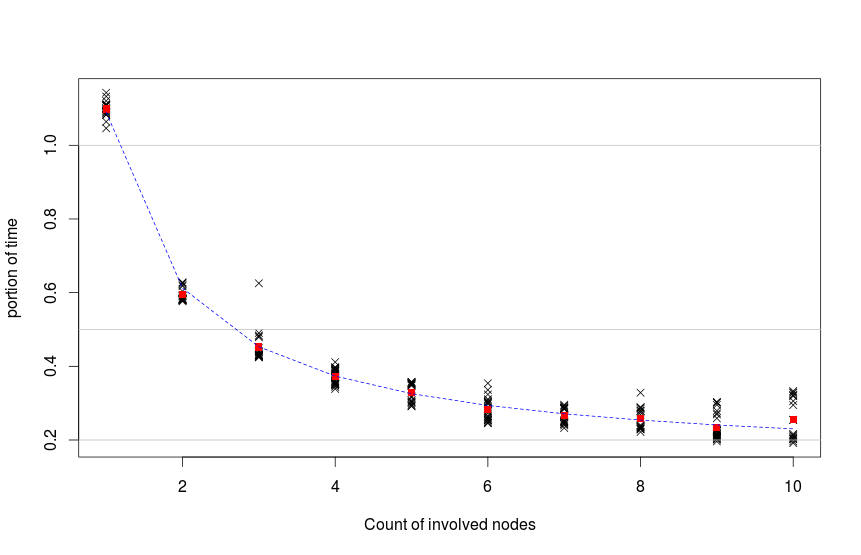
\includegraphics[scale=0.45]{./img/improvement_root.png}
\caption{Achieved improvement - all measurements}
\end{center}
\end{figure}

The figures 3.2 - 3.4 shows the achieved speedup. The y-axis shows the
obtained speedup. Model that was used is further described in the next
section. The data are represented by gray crosses, the estimation based
on the model is visualized by the blue dashed line. The red line shows
the linear function, which would be the ideal case. This linear function
is of the form

\begin{center}
$y = q*x$
\end{center}

where coefficient \textit{q} represents the influence of the time
consumed by the data transfers. The Figure 3.4 shows, that for this
chunk size the time spent with the distribution causes latency when more
nodes are employed. This is caused by the fact, that too many transfers
are processed in parallel. Consequently, some of the nodes have to wait
for the chunks for too long.

\begin{figure}[h]
\begin{center}
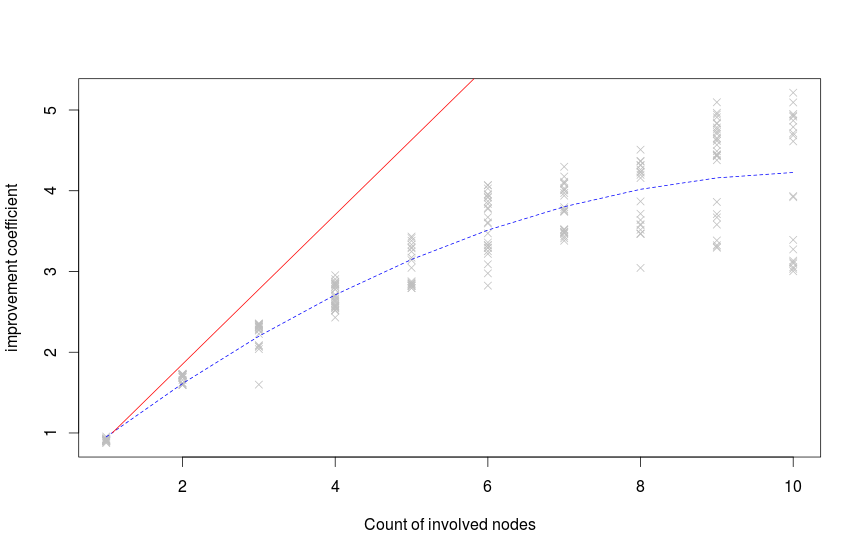
\includegraphics[scale=0.45]{./img/Rplot_all.png}
\caption{Achieved speedup - all measurements}
\end{center}
\end{figure}

\begin{figure}[h]
\begin{center}
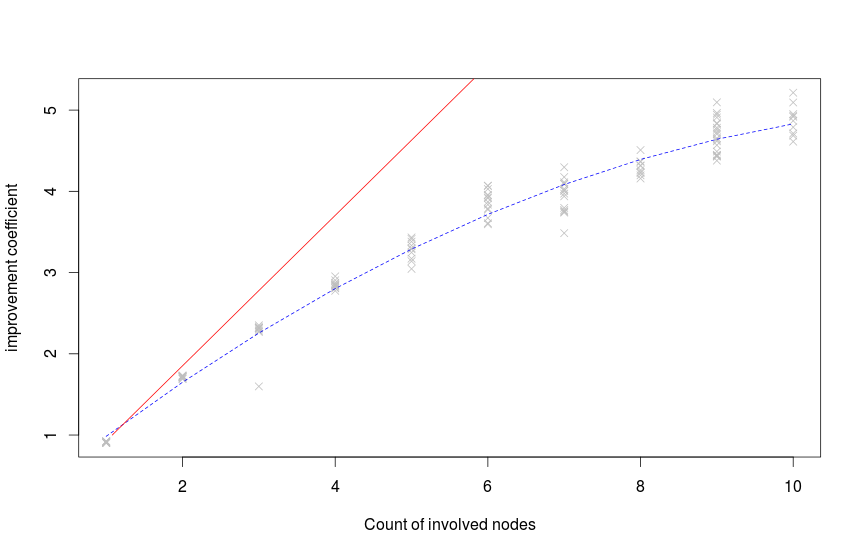
\includegraphics[scale=0.45]{./img/Rplot10k.png}
\caption{Achieved speedup - 10 MB chunks}
\end{center}
\end{figure}

\begin{figure}[h]
\begin{center}
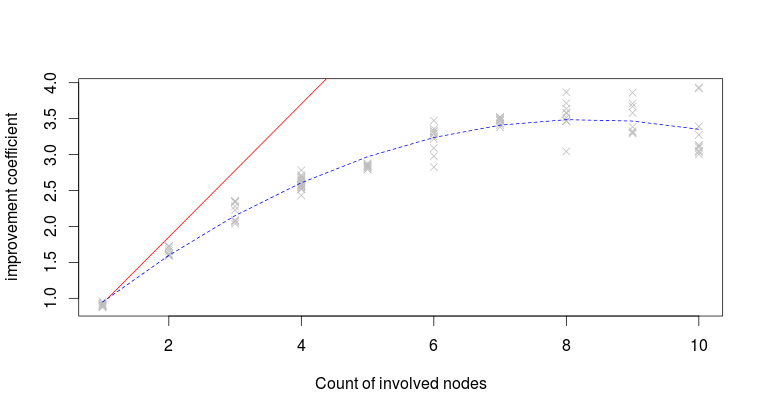
\includegraphics[scale=0.45]{./img/Rplot40k.png}
\caption{Achieved speedup - 40 MB chunks}
\end{center}
\end{figure}

In the Figures 3.5 and 3.6 are displayed ratios between particular
operations performed during the process. The ratios are displayed with
respect to the time that would be taken by the serial execution. Each
column represents one measurement (process). The first image displays
data for chunks with 10 MB in size, the second shows 40 MB chunks. The
data are sorted according to the number of neighbors used in the
process. We can see that portion of time spent with network transfers is
relatively small in our case. These charts were generated using the
LibreOffice package\footnote{http://www.libreoffice.org/}

\begin{figure}[h]
\begin{center}
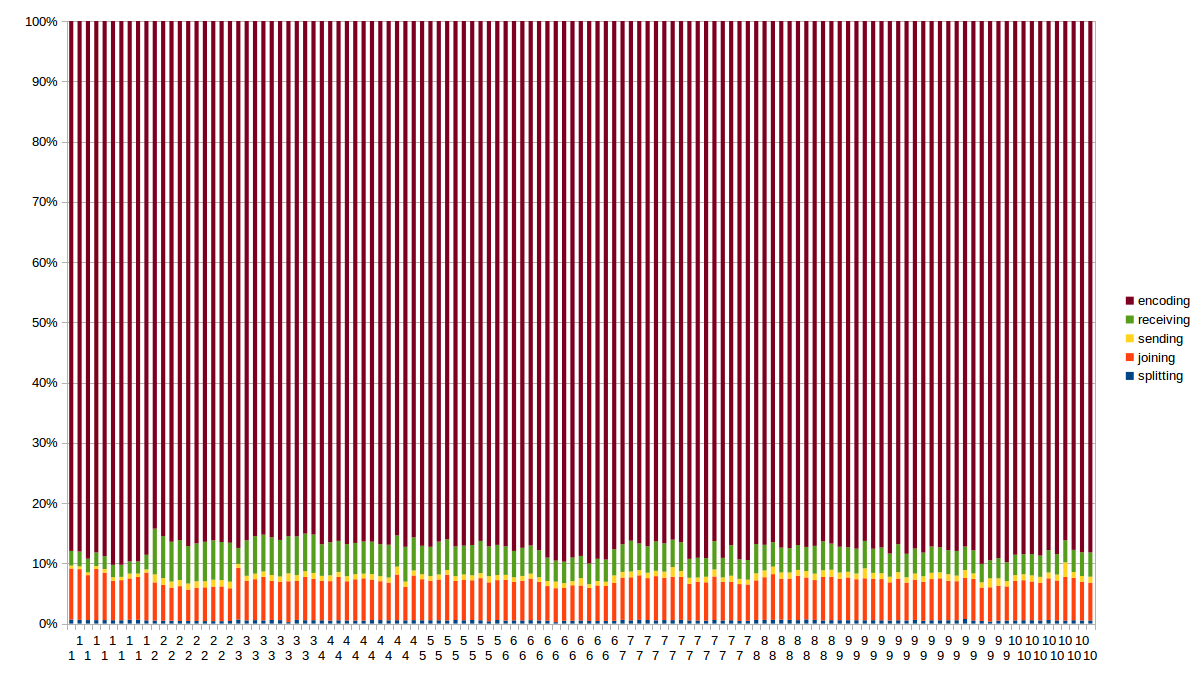
\includegraphics[scale=0.5]{./img/comparison_chart.png}
\caption{Comparison of operation times - 10 MB chunks}
\end{center}
\end{figure}

\begin{figure}[h]
\begin{center}
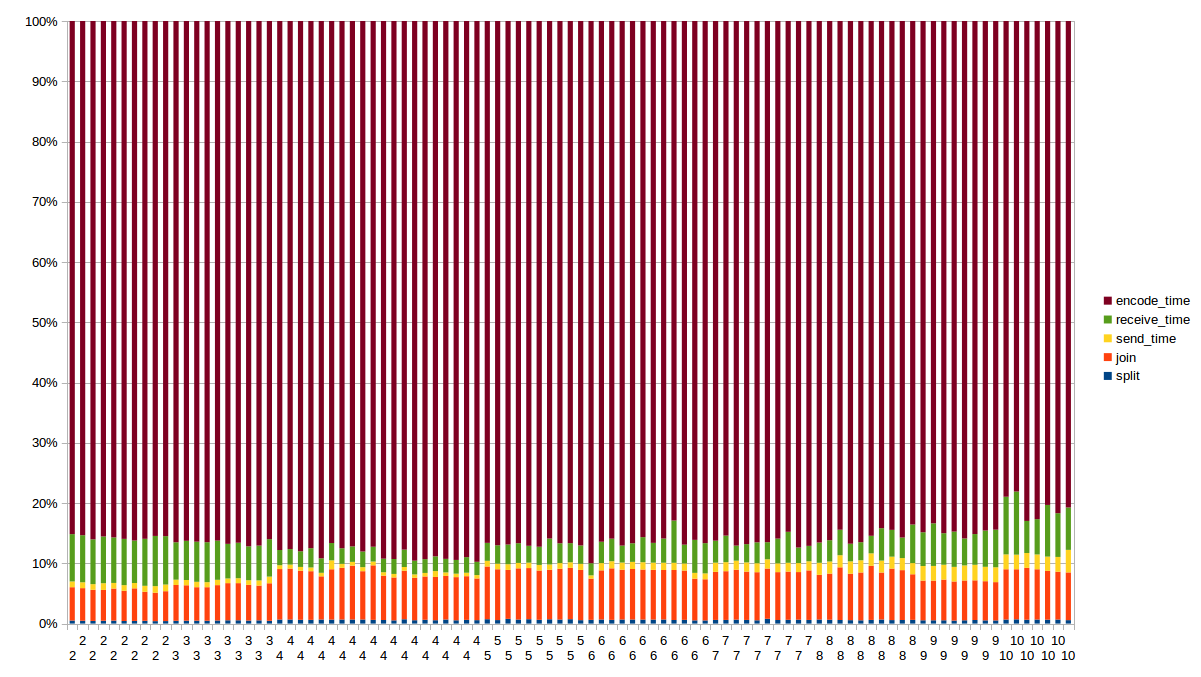
\includegraphics[scale=0.5]{./img/comparison_chart40k.png}
\caption{Comparison of operation times - 40 MB chunks}
\end{center}
\end{figure}

Figure 3.7 shows results of the experiment, in which one of the nodes
was killed during the process and then spawned again. As a result,
several chunks were sent more times, depending on the conditions in the
network. The plot shows average number of chunk sent and achieved
improvement. In this experiment, 40 MB chunks were used, displayed in
the left side. Also, some of the experiments were intentionally run with
no failure, so we can see results achieved with normal run in the left
down corner and we can compare it. Those values are highlighted. We can
see, that resending of chunks has great impact on the result. This
problem could be reduced by using smaller chunks. When we used 5 MB
chunks, the results improved significantly as showed in the right image
in the Figure. This is caused by the fact, that with the same number of
faults, the amount of work that needs to be done again is smaller when
using smaller chunks. However, disadvantage of this approach is, that
the split and join operations take slightly more time.

\begin{figure}[h]
\begin{center}
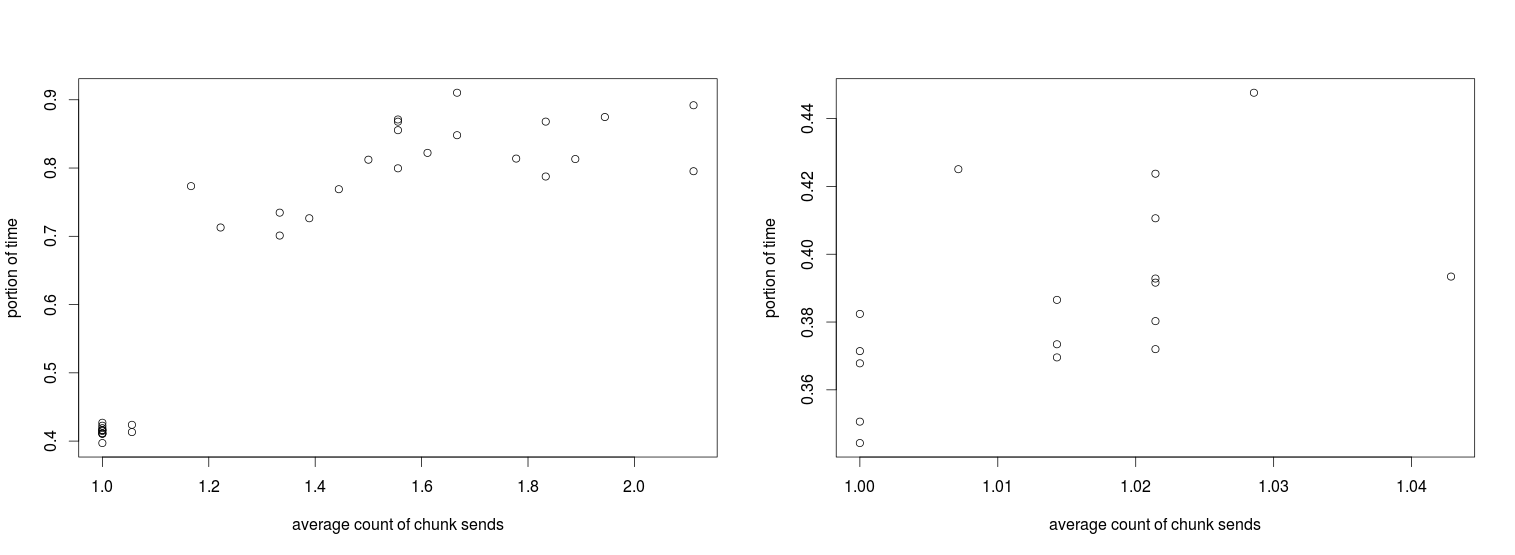
\includegraphics[scale=0.30]{./img/failures_both.png}
\caption{Impact of resending on the result}
\end{center}
\end{figure}

\pagebreak

\subsection{Linear Model}\label{linear-model}

Work with the data and the model was performed in the R Studio
program\footnote{https://www.rstudio.com/}. To evaluate the data, simple
linear regression model was used. Specifically, subsequent formula was
used:

\begin{center}
$\frac{single\_node\_time}{distributed\_time} = \beta_0 + \beta_1 \times neighbor\_count + \beta_2 \times neighbor\_count^2 + \epsilon_i$
\end{center}

Higher powers were not used in order to not over fit the model. The
analysis of the model showed, that it makes sense to use this model. The
assumptions such as homoscedasticity (constant variance) and
independence of errors were explored using plots and results given by
the R Studio. Some of the mentioned outputs are given in the Figures 3.8
and 3.9. We can see, that according to the p-values corresponding to
coefficients, all of them are significant for the model. Residual
standard error shows, that the variance is not too big. In the plots we
can see that the residuals unfortunately has not constant variance. The
second plot also suggests, that they probably are not distributed
normally. However, citation says: ``heteroscedasticity has never been a
reason to throw out an otherwise good model.''\citep{ECON} So we used
this model in our modeling. It may be questionable, whether we had
enough measurements, however, the model seems to be good enough to
describe the data and predict the behavior for more nodes. We can also
notice, that the $\beta_2$ coefficient is negative and since the squared
value rises faster, there is some point at which the improvement stops
raising, which corresponds to reality.

\begin{figure}[h]
\begin{center}
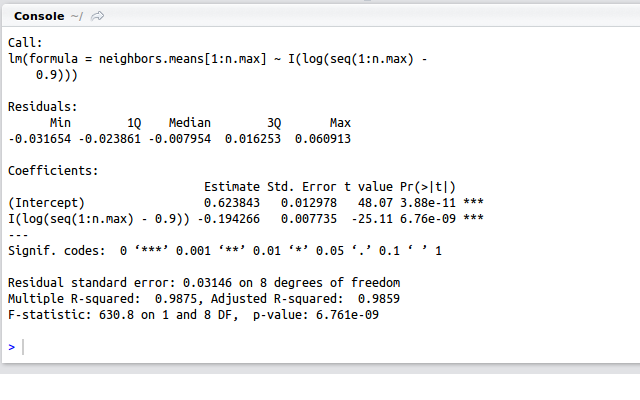
\includegraphics[scale=0.60]{./img/model.png}
\caption{Summary of the model}
\end{center}
\end{figure}

\begin{figure}[h]
\begin{center}
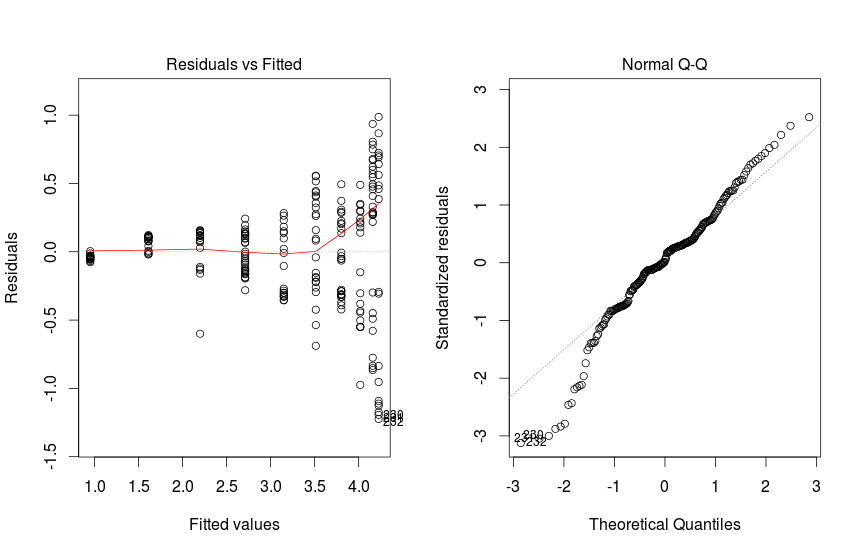
\includegraphics[scale=0.45]{./img/model_plots.png}
\caption{Graphical representation of the model data}
\end{center}
\end{figure}

\subsection{Upper Bounds}\label{upper-bounds}

Overall time of the process can be divided into operations split, send,
encode, receive and join (in this order). It is also influenced by
searching appropriate neighbors, but it will not be taken into account
in this analysis. Also, based on the data we can observe, that the time
taken by the split operation is not very significant, therefore we can
omit it. If we ask how big speedup can be achieved, we can use the
Amdahl's law\footnote{https://en.wikipedia.org/wiki/Amdahl's\_law} to
model the situation. The join operation can not be parallelized. The
encoding itself is parallelized completely. The data transfer operations
are performed theoretically in parallel, however, in practice we are
limited by the network throughput and the system resources of the
initiator, i.e.~how many data transfers it can handle in parallel. This
can be influenced by the OS, disk speed or even operation memory.
Because this number is limited, the initiator can not employ arbitrary
number of nodes effectively. If we want to deal with this problem, we
have to consider several facts. The speed of the distribution is
influenced by the ability of the nodes to receive the data with no
delay, so we assume that buffering and disk operations do not slow down
the process. Also, the full network capacity cannot be used because of
other ongoing transfers. Some portion of the capacity is consumed by the
redundant information used by the TCP/IP too. For the sake of
simplicity, we will make the assumption, that the capacity corresponds
to the actual amount of useful data transfered. We also must not forgot,
that the sizes of original and received chunks differs. Finally, we
treat the parallel transfer over the network as it took the same time as
the serial, which does not have to be always true. We will consider the
size of received chunks to be $k$ times bigger than the size of the send
ones and count with this size. Let $c$ be the amount of data that can be
transfered over the network per one second, $s$ chunk size and $t$ time
needed to encode one chunk (here we assume the encoding times are the
same for all the nodes). Then maximum number $n$ of effectively employed
nodes must fulfill the inequality:

\begin{center}
$\frac{n \times s}{c} \leq t$
\end{center}

since otherwise the transfer would take more time than the encoding, so
the encoded chunks would have to wait.

To applicate the Amdahl's law, we must determine the fraction of the
algorithm that is strictly serial. This involves the splitting and
joining. We consider the data transfers to be parallelized with the
preceding paragraph in mind. According to the results, the split and
join operations take approximately 7.5\% of time in average. So
according to the basic form of the law, the theoretical maximum speedup
should be obtained from the following formula:

\begin{center}
$S=\lim_{n \to +\infty} \frac{1}{B + \frac{1}{n}(1 - B)} = \frac{1}{B} = \frac{1}{0.075} = 13.33$
\end{center}

Where $B$ represents the serial fraction. This result is strictly
theoretical and does not correspond to real situation, mainly because of
the problems mentioned above. We can obtain more realistic results by
using the formula to estimate the parallel fraction of time.

\begin{center}
$P_{est} = \frac{\frac{1}{speedup}-1}{\frac{1}{node count} - 1}$
\end{center}

For our data the estimation equals $0.89$, which gives us theoretical
maximum speedup $9.09$.
\chapter{Problems, alternatives and possible
improvements}\label{problems-alternatives-and-possible-improvements}

Some alternative approaches were also considered during the designing.
One of them was not to use periodical checking at all. It was based on
the idea, that there would exist permanent connection with each neighbor
and the state changes would be indicated by the events related to this
connection. However it was rejected due to the requirements connected
with keeping the connection. Furthermore, the changes of ready state of
the node would have to be checked either periodically or the node would
have to inform all its neighbors (even potential) about each change
which would lead to another problems to deal with. It is in contrast
with passivity of the slaves too.

Another issue was related to more sophisticated way of distributing the
chunks. Namely some kind of hierarchy was considered in which the chunk
references would be distributed to neighbors in packs. At the neighbor
it would be further split and distributed among neighbor's neighbors and
so on. A kind of a tree structure would be formed this way. The transfer
of the file would be processed directly between the initiator and the
leaf node. However this approach turned out to be complicated and brings
many problems. For example in case of failure of some node which is high
in the hierarchy a lot of chunks would have to be re-distributed. Also
the initiator's ability to control the distribution would be reduced.
Moreover, the advantages of this approach are not so significant at all,
because the biggest portion of time is spent during transfers and
processing the chunks. The time spent with distribution of references is
not important at all.

Interesting alternative would be use of the
anycast\footnote{https://en.wikipedia.org/wiki/Anycast} mechanism
provided by the IPv6 protocol. The nodes would be addressed with an
anycast address and each chunk would be simply sent to this address.
Obvious disadvantage of this approach is the loss of the control of the
distribution. More sophisticated variant would use special node which
would maintain the list of free nodes and schedule the distribution.
However this would break the peer to peer paradigm because of the
centralization of control to one specific node.

Maybe the biggest unnecessary delay could appear when the whole process
waits for some lost chunk. This is partially solved by resending chunks
after the timeout. Also some form of redundancy could help, which on the
other hand would certainly affect the effectiveness. If some node is
processing more tasks sequentially while using approximately the same
set of neighbors, the framework could also determine optimal chunk size
to achieve good ratio of transfer and computing times. The chunks should
not be too small because of the delays tied with its distribution.
Optimal chunk size could significantly reduce the possible delay caused
by waiting for re-encoding of some lost chunk. We could see at the end
of the \hyperref[interpreting-the-results]{chapter 3}, that use of
smaller chunk size leads to better performance, especially when the
failure of some node occurs, the difference can be quite big.

Also the current implementation creates a separate connection for each
data transfer. Alternatively, each chunk could be delivered and returned
using the same connection which would lessen the demands of the
communication. The connection's termination would also indicate problem
with the chunk's processing or the neighbor itself. But the connection
termination does not necessarily mean the failure of the process.
Because it is desirable to avoid needless re-encoding of the chunks,
this situation would has to be treated specially which would introduce
additional problems. Also this approach does not fit very well to the
current design in which each logical action is executed as the sequence
of commands and for each sequence there is a special connection.
 
% An example of LaTeX use (uncomment, if you wish)
% %%% Ukázka použití některých konstrukcí LaTeXu

\subsection{Ukázka \LaTeX{}u}
\label{ssec:ukazka}

This short subsection serves as an~example of basic \LaTeX{} constructs,
which can be useful for writing a~thesis.

Let us start with lists:

\begin{itemize}
\item The logo of Matfyz is displayed in figure~\ref{fig:mff}.
\item This is subsection~\ref{ssec:ukazka}.
\item Citing literature~\cite{lamport94}.
\end{itemize}

Different kinds of dashes:
red-black (short),
pages 16--22 (middle),
$45-44$ (minus),
and this is --- as you could have expected --- a~sentence-level dash,
which is the longest.
(Note that we have follwed \verb|a| by a~tilde instead of a~space
to avoid line breaks at that place.)

\newtheorem{theorem}{Theorem}
\newtheorem*{define}{Definition}	% Definice nečíslujeme, proto "*"

\begin{define}
A~{\sl Tree} is a connected graph with no cycles.
\end{define}

\begin{theorem}
This theorem is false.
\end{theorem}

\begin{proof}
False theorems do not have proofs.
\end{proof}

\begin{figure}
	\centering
	
\includegraphics[width=30mm]{../img/logo.eps}
	\caption{Logo of MFF UK}
	\label{fig:mff}
\end{figure}


\chapter*{Conclusion}
\addcontentsline{toc}{chapter}{Conclusion}
Based on the experiments it can be said, that the framework works fine and it can be successfully used to speed up computation in the local network. Although the achieved speed up does not grow linearly with the increasing number of nodes, it can be quite significant. It was not tested in WAN environments, however, according to the results, the transfers of the data takes indispensable portion of the whole processing time, so the improvement depends on the network throughput. 

As is being discussed in \hyperref[Problems-alternatives-and-possible-improvements]{chapter 4}, the framework could be further improved. To achieve more effective distribution of the work, more sophisticated scheduling could be employed. Also it was shown, that some redundancy for prevention of re-computing whole node could be useful. Because of the speed of the network the data transfers generally seems to be a bottleneck, so good scheduling algorithm appears to be very important, together with optimal choice of the chunk size. This leads us to a conclusion, that in reliable network environments is probably better idea to centralize logic to special node in order to achieve better performance and accept potential malfunctions caused by the control node failure.

\chapter*{Appendix A - Installation and use}
\section{Download} 
First it's essential to get the source code. You can clone the code directly from the git repository using command
\begin{verbatim}
# git clone https://github.com/vojtsek/VideoCompression.git
\end{verbatim}
Alternatively you can download the zip file and unpack it in some directory.

\section{Requirements, installation and first run}
To run the program successfully it's essential to have \textit{ffmpeg} and \textit{ffprobe} installed on your computer. Although technically it doesn't matter which codec is used, the program currently uses only H.264 standard for encoding of the output, so it assumes the \textit{ffmpeg} has been compiled with the \textit{x264} codec. Otherwise the program does not have any special requirements except standard libraries which should be available on all UNIX systems, so once you installed these programs, you can change to the directory containing the source code and run the installation script:
\begin{verbatim}
# cd DVC
# ./install.sh
\end{verbatim}
The installation script is a regular Bash script, so the Bourne again shell interpreter is required to run it successfully. It explores your computer, i.e. gets the IP address, finds location of \textit{ffmpeg} binaries etc. Then it creates home directory for the program. The home directory contains data of the program's run. These include intermediate results as well as the final result and log files. The installation continues with generating the configuration file. This file is crucial for the framework. Before setting each option, the script prompts you for confirmation of the value. If you type nothing and just press the Enter key, the suggested value is used, otherwise the script uses your input. The resulting file is stored in the \textit{bin} directory which is created during the installation. It's a plain text file so you can edit it anytime in the future. The script then continues with compilation of the program. If everything is all right, you can change to the newly created \textit{bin} directory and continue. The directory \textit{bin/lists} contains some supporting files that should not be change, otherwise the program could behave improperly.

The last step before you can run the program is to check the configuration. The configuration is saved in the \textit{bin/CONF} file, which is created by the installation script. It's important to provide valid path to the \textit{ffmpeg} and \textit{ffprobe} executable and address with port of the neighbor that should be contacted initially. Otherwise you won't be able to join the network. The field \textit{MY\_IP} is not essential as long as the initial neighbor is alive - it will be recognized automatically. 

Then you can finally run the program. Some of the settings can be changed by providing options, the available ones are listed in the table 4.1.

\begin{table}[h]
\begin{center}
 \begin{tabular}{ | l | c |}
   \hline
-s & no address will be contacted initially \\ \hline
-n [address]:port\_number & node to contact initially \\ \hline
-a [address]:port\_number & address and port to bound to \\ \hline
-h & directory path to the home directory \\ \hline
-i file & file to encode \\ \hline
-p port & listening port \\ \hline
-d level & debug level \\ \hline
-q quality & quality of encoding \\ \hline
 \end{tabular}
 \caption{Table of the possible options.}
 \end{center}
\end{table}

If the string "\textit{IPv4}" appears among parameters, the program will use only the IPv4 addresses\footnote{https://en.wikipedia.org/wiki/IPv4},
in which case should be the \textit{CONF} file changed appropriately.

\section{Using the program}
When you run the program, the initial screen appears. You can choose desired action then using function keys. You can see the initial screen in the figure 4.1. Available options are highlighted.
\begin{figure}[h]
\begin{center}
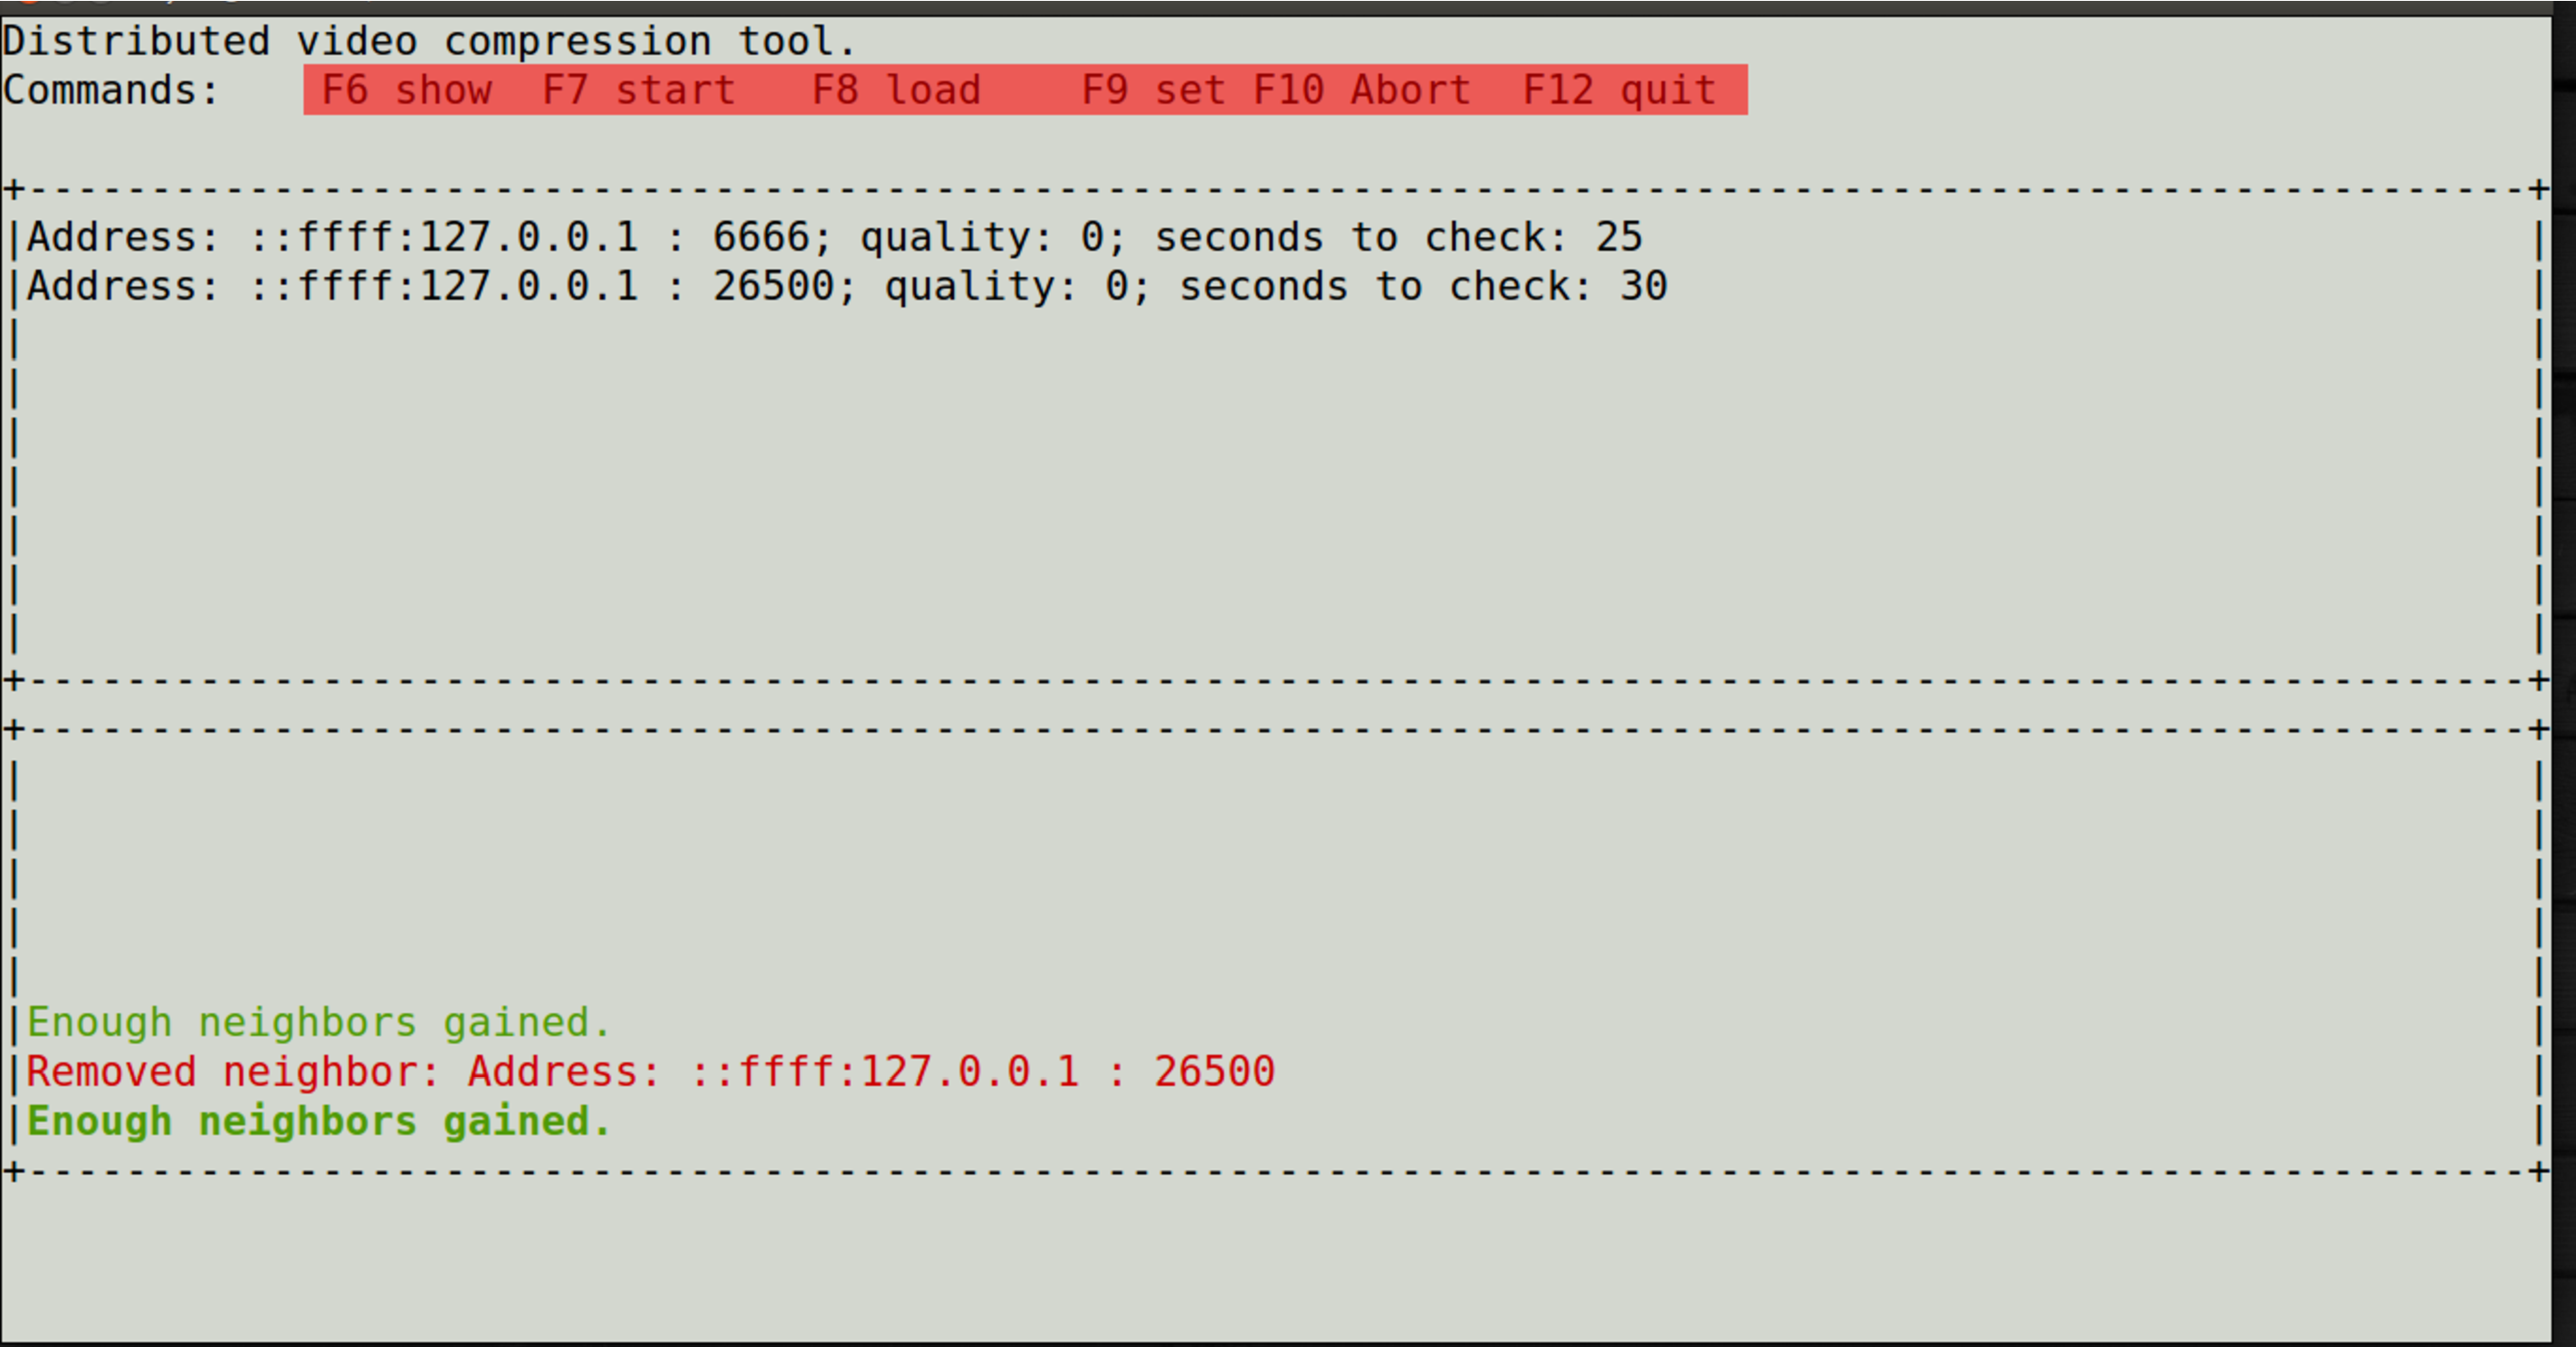
\includegraphics[scale=0.35]{./img/init-screen.pdf}
\label{initial-screen}
\caption[initial-screen]{Initial screen after joining.}
\end{center}
\end{figure}

The important key bindings are listed in the table 4.2.
\begin{table}[h]
\begin{center}
 \begin{tabular}{ | l | c |}
   \hline
   F6 & Show information \\ \hline
   F7 & Start the process \\ \hline
   F8 & Load the file \\ \hline
   F9 & Set values \\ \hline
   F10 & Abort the process \\ \hline
   F12 & Quit the program \\ \hline
   Up, Down & Traverse available options \\ \hline
   Enter & Confirm the input \\
 	\hline
 \end{tabular}
 \caption{Table of the control keys.}
 \end{center}
\end{table}

First you should load the video file. When the corresponding function key is pressed, the program prompts you for the file location. You can type in the absolute path of the file. Once you use the file, it is stored in history which you can browse using up and down arrow keys. This can be seen in the figure 4.2.
\begin{figure}[h]
\begin{center}
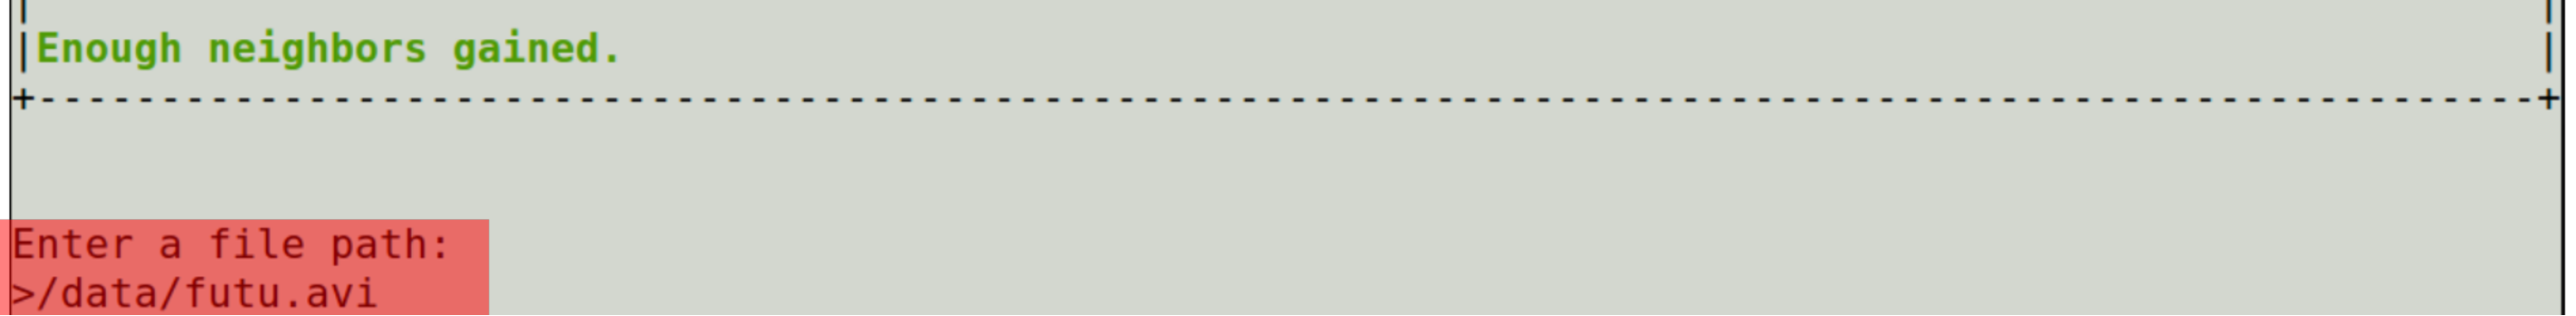
\includegraphics[scale=0.35]{./img/loading.pdf}
\label{loading-files}
\caption{Loading the file.}
\end{center}
\end{figure}

Then you can set some parameters or show different information using F6 respectively F9 function keys. These keys provides set of options which you can choose from. When you are satisfied with the settings, you can start the process.
The program then starts splitting the file and distributing the chunks while informing you about the progress. When the process is done, the file is joined and you can do further actions. Some screenshots from the ongoing process are displayed at the figures 4.3, 4.4 and 4.5
\begin{figure}[h]
\begin{center}
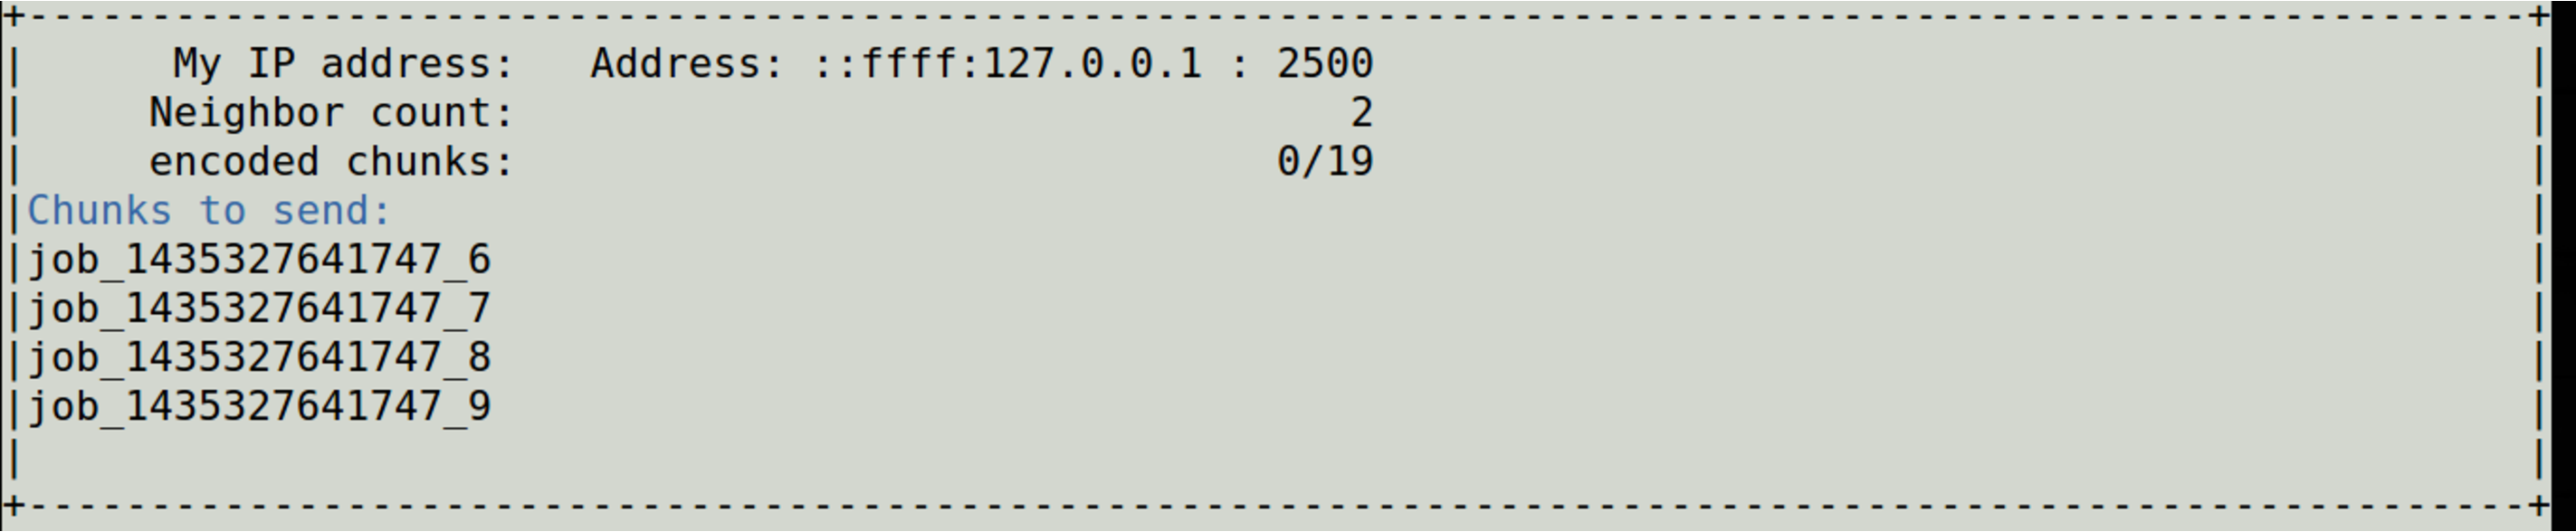
\includegraphics[scale=0.35]{./img/process-initiator.pdf}
\caption{Overview of the process.}
\end{center}
\end{figure}
\begin{figure}[h]
\begin{center}
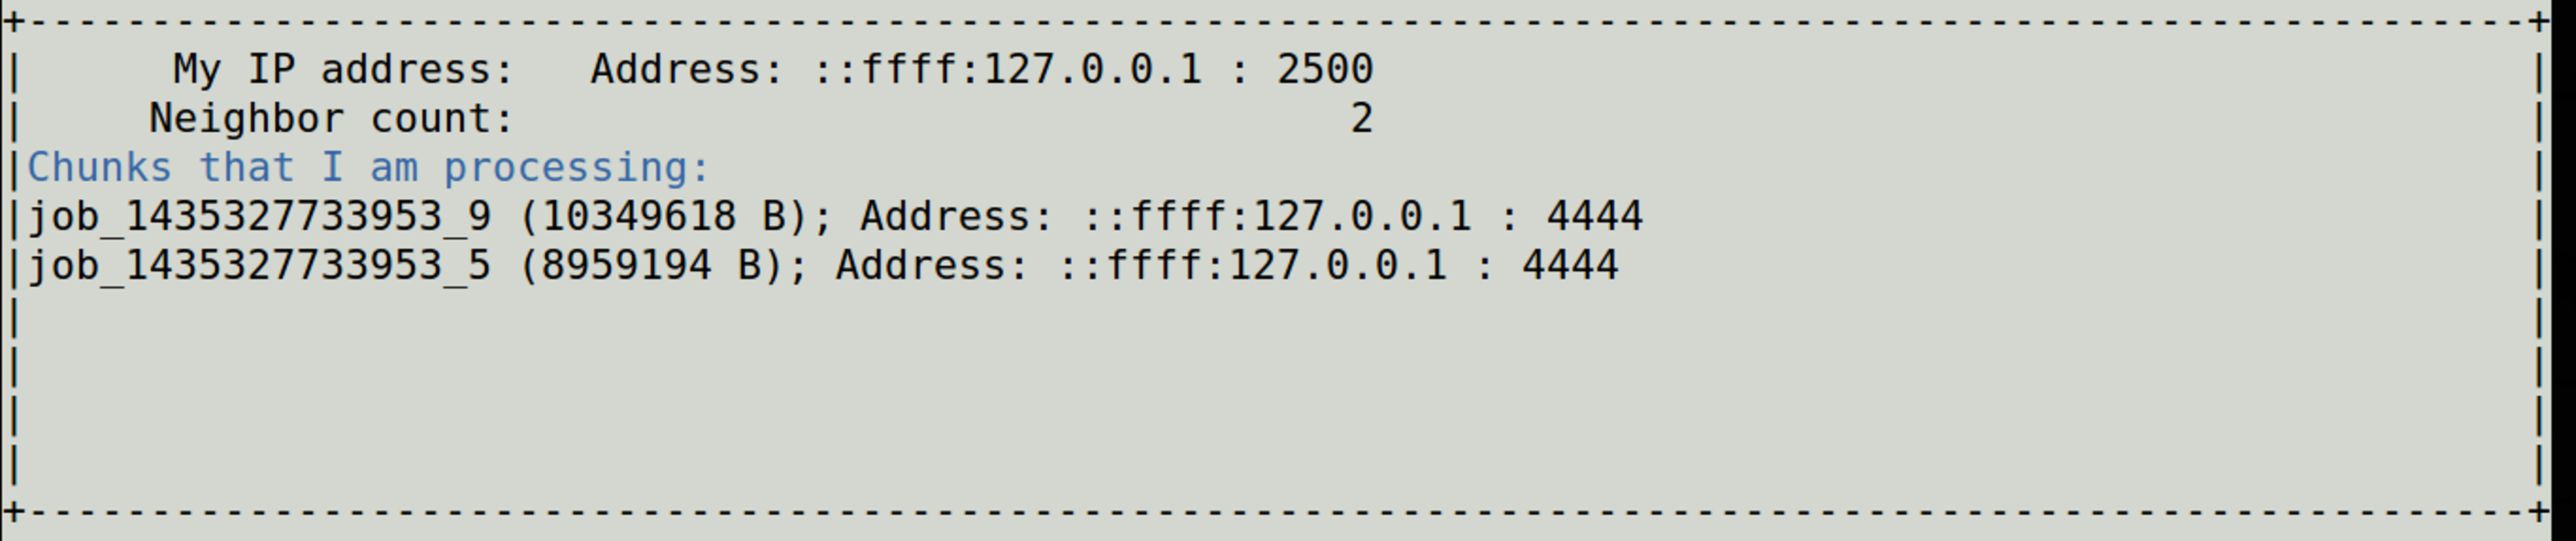
\includegraphics[scale=0.35]{./img/processing.pdf}
\caption{Processing of the tasks.}
\end{center}
\end{figure}
\begin{figure}[h]
\begin{center}
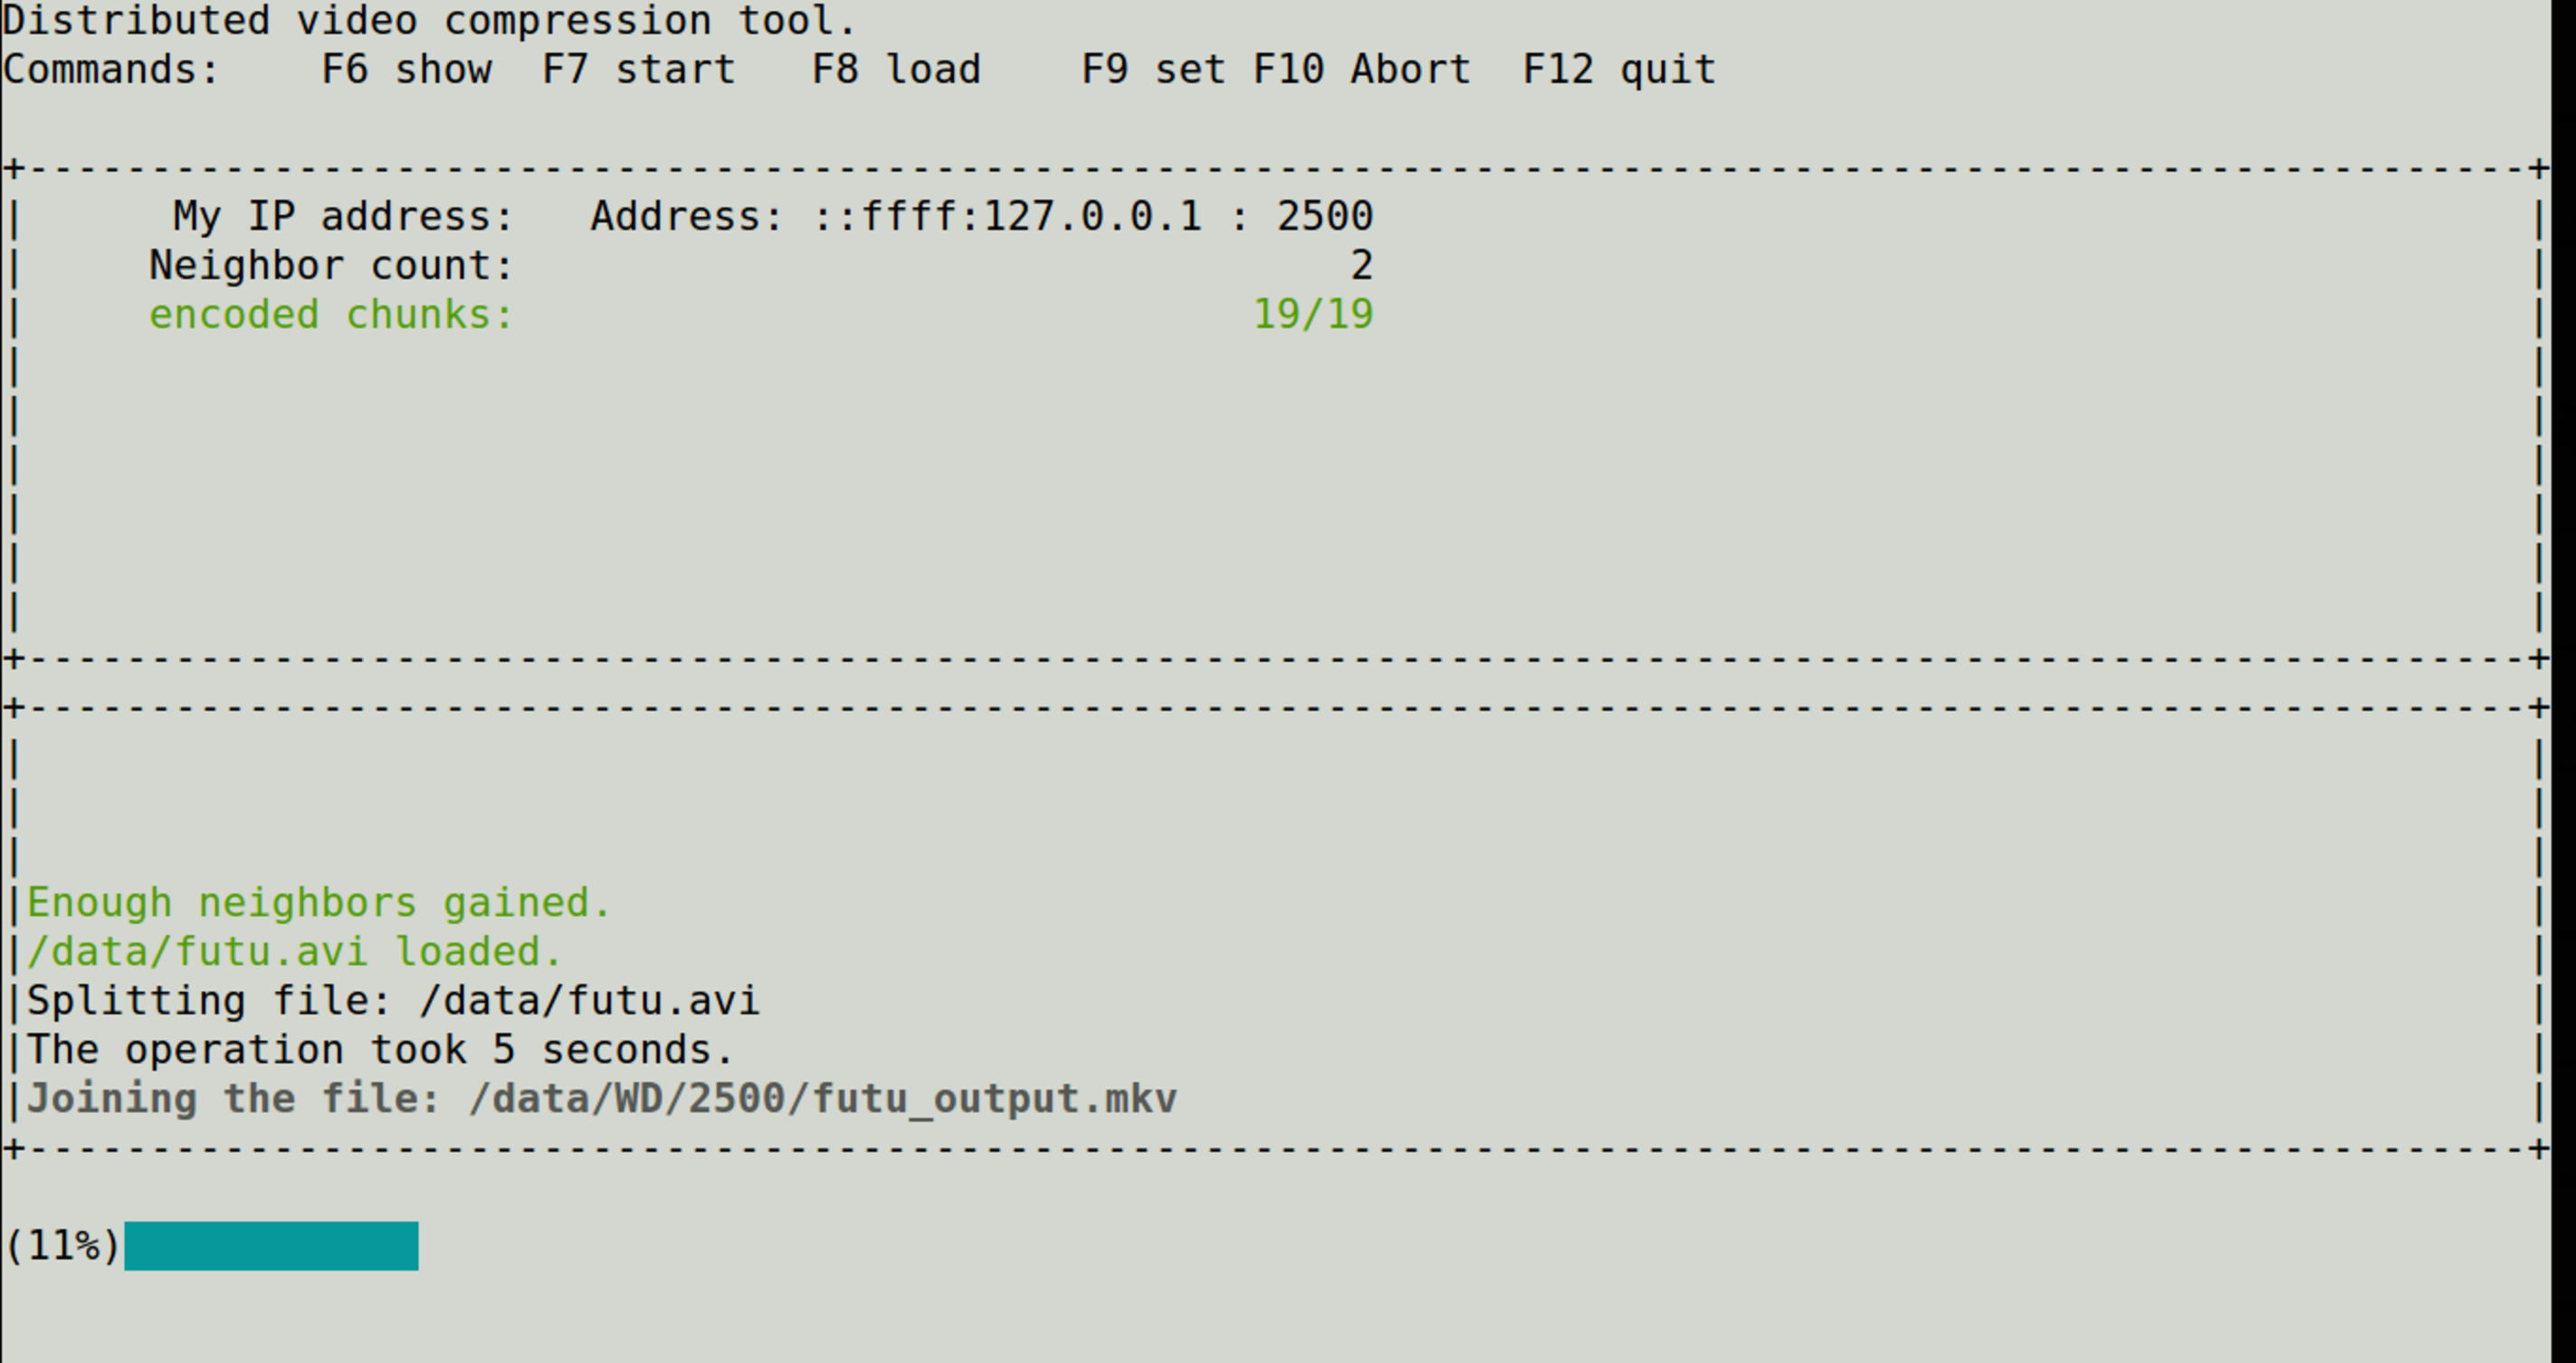
\includegraphics[scale=0.35]{./img/joining.pdf}
\caption{Joining the file.}
\end{center}
\end{figure}

To obtain more information about what is going on, the \textit{-d} option may be used which allows to specify level of debug messages that will be shown.

%%% Bibliography
\bibliographystyle{csplainnat}
\bibliography{literature}
\addcontentsline{toc}{chapter}{\bibname}

%%% Figures used in the thesis (consider if this is needed)
\listoffigures

%%% Tables used in the thesis (consider if this is needed)
\listoftables

%%% Abbreviations used in the thesis, if any, including their explanation
\chapwithtoc{List of Abbreviations}
\begin{itemize}
\item \textbf{LAN} Local Area Network
\item \textbf{TCP} Transmission control protocol
\item \textbf{IPv4 (IPv6)} Internet Protocol version 4 (version 6)
\item \textbf{API} Application programming interface
\item \textbf{GUI} Graphical User Interface
\item \textbf{HTML} Hypertext Markup Language
\item \textbf{OS} Operating System
\item \textbf{STL} Standard Template Library
\item \textbf{JSON} JavaScript Object Notation
\item \textbf{MTU} Maximum Transmission Unit
\item \textbf{B, kB, MB, GB} Byte, kiloByte, megaByte, gigaByte
\end{itemize}

%%% Attachments to the bachelor thesis, if any (various additions such
%%% as programme extracts, diagrams, etc.). Each attachment must be referred to
%%% at least once from one's own text of the thesis. Attachments are numbered.
\chapwithtoc{Attachments}

\section*{Appendix A - Installation and use}
\subsection*{Download} 
First it's essential to get the source code. You can clone the code directly from the git repository using command
\begin{verbatim}
# git clone https://github.com/vojtsek/VideoCompression.git
\end{verbatim}
Alternatively you can download the zip file and unpack it in some directory.

\subsection*{Requirements, installation and first run}
You must have \textit{ffmpeg} and \textit{ffprobe} installed on your computer, if you want to run the program successfully. Although technically it doesn't matter which codec is used, the program currently uses H.264 standard as a default, so it assumes the \textit{ffmpeg} has been compiled with the \textit{x264} codec support. Otherwise the program does not have any special requirements except standard libraries which should be available on all UNIX systems. When you install these programs, you can change to the directory containing the source code and run the installation script:
\begin{verbatim}
# cd VideoCompression
# ./install.sh
\end{verbatim}
The installation script is a regular Bash script, so the Bourne again shell interpreter is required to run it successfully. It uses utilities that are common part of every Linux distribution. If some of it is not present, you can either install it or do the preparation yourself. The script explores your computer, i.e. gets the IP address, finds location of \textit{ffmpeg} binaries etc. Then it creates home directory for the program. The home directory contains data of the program's run. These include intermediate results as well as the final result and log files. The installation continues with generating the configuration file. This file is crucial for the framework. Before setting each option, the script prompts you for confirmation of the value. If you type nothing and just press the \textit{Enter} key, the suggested value is used, otherwise the script uses your input. The result configuration file is stored in the \textit{bin/} directory which is created during the installation. It's a plain text file so you can edit it anytime in the future. The script then continues with compilation of the program. If everything is all right, you can change to the newly created \textit{bin/} directory and continue. The directory \textit{bin/lists/} contains some supporting files that should not be changed. Otherwise the program could behave improperly.

The last step before you can run the program is to check the configuration. The configuration is saved in the \textit{bin/CONF} file, which is created by the installation script. It's important to provide valid path to the \textit{ffmpeg} and \textit{ffprobe} executables and address with port of the neighbor that should be contacted initially. Otherwise you won't be able to join the network. The field \textit{MY\_IP} is not essential as long as the initial neighbor is alive - it will be recognized automatically. 

Then you can finally run the program. Some of the settings can be changed by providing options, the available ones are listed in the table 4.1.

\begin{table}[h]
\begin{center}
 \begin{tabular}{ | l | c |}
   \hline
-s & no address will be contacted initially \\ \hline
-n [address]:port\_number & node to contact initially \\ \hline
-a [address]:port\_number & address and port to bound to \\ \hline
-h & directory path to the home directory \\ \hline
-i file & file to encode \\ \hline
-p port\_number & listening port \\ \hline
-d level & debug level \\ \hline
-q quality & quality of encoding \\ \hline
 \end{tabular}
 \caption{Table of the possible options.}
 \end{center}
\end{table}

If the string \textit{IPv4} appears among parameters, the program will use only the IPv4 addresses\footnote{https://en.wikipedia.org/wiki/IPv4},
in which case should be the \textit{CONF} file changed appropriately.

\subsection*{Using the program}
When you run the program, the initial screen appears. You can perform desired action using function keys. You can see the initial screen in the Figure 4.1. Available options are highlighted.
\begin{figure}[h]
\begin{center}
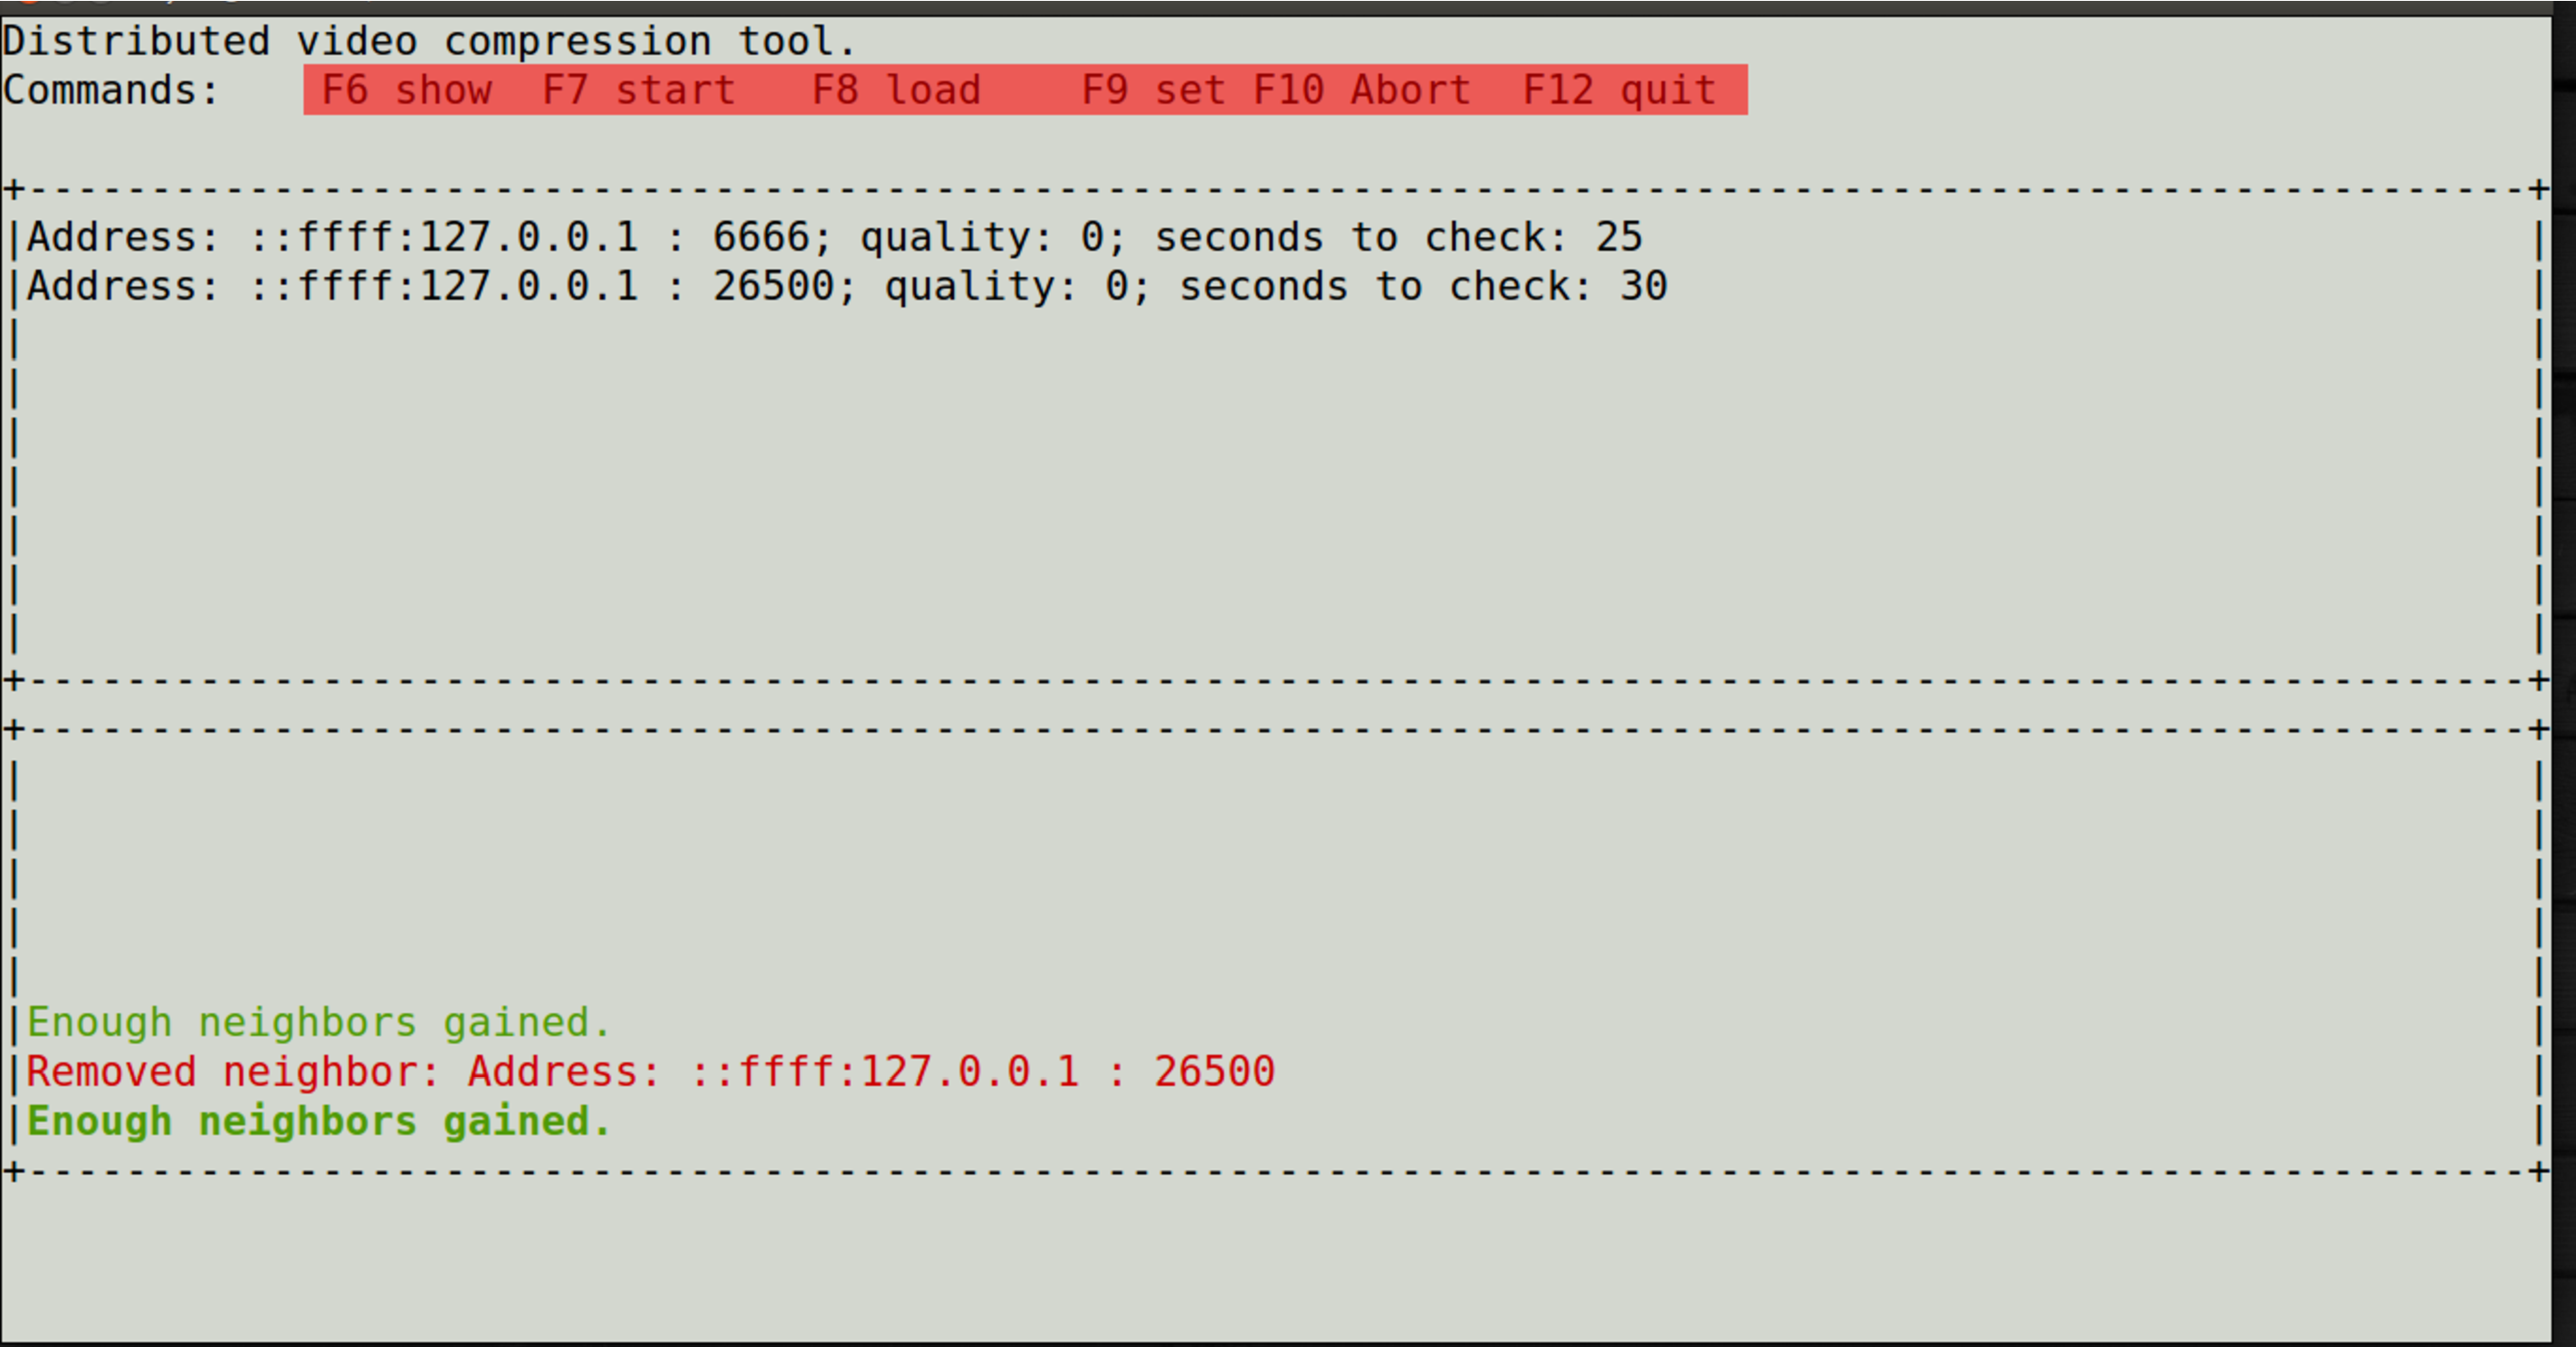
\includegraphics[scale=0.30]{./img/init-screen.pdf}
\label{initial-screen}
\caption[initial-screen]{Initial screen after joining.}
\end{center}
\end{figure}

The important key bindings are listed in the table 4.2.
\begin{table}[h]
\begin{center}
 \begin{tabular}{ | l | c |}
   \hline
   F6 & Show information \\ \hline
   F7 & Start the process \\ \hline
   F8 & Load the file \\ \hline
   F9 & Set values \\ \hline
   F10 & Abort the process \\ \hline
   F12 & Quit the program \\ \hline
   Up, Down & Traverse available options \\ \hline
   Enter & Confirm the input \\
 	\hline
 \end{tabular}
 \caption{Table of the control keys.}
 \end{center}
\end{table}

First you should load the video file. When the corresponding function key is pressed, the program prompts you for the file location. You can type in the absolute path of the file. Once you use the file, it is stored in history which you can browse using up and down arrow keys. This can be seen in the Figure 4.2.
\begin{figure}[h]
\begin{center}
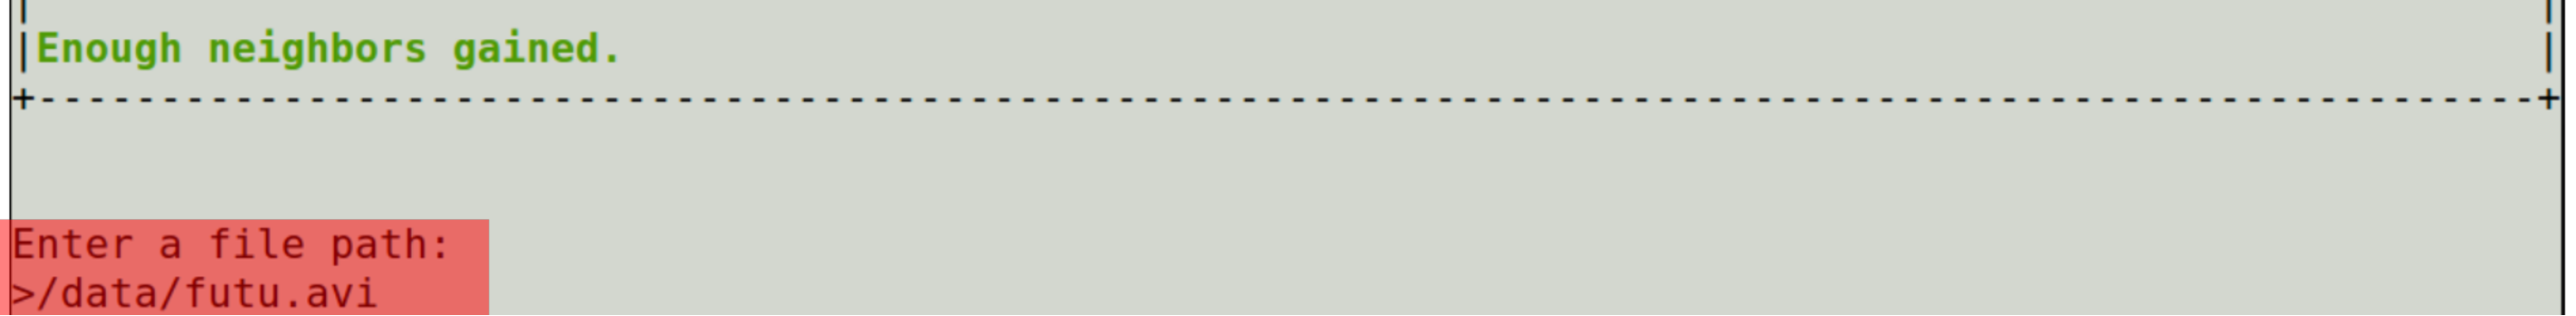
\includegraphics[scale=0.30]{./img/loading.png}
\caption{Loading the file.}
\end{center}
\end{figure}

Then you can set some parameters or show different information using F6 respectively F9 function keys. These keys provides set of options which you can choose from. When you are satisfied with the settings, you can start the process.
The program then starts splitting the file and distributing the chunks. It also keeps informing you about the progress. When the process is done, the file is joined and you can do further actions. You can find the result in the provided work directory. There should appear new folder with a timestamp of the current job. It contains the file named \textit{orig\_output.mkv}, where \textit{orig} is the base name of the input file. Some screenshots from the ongoing process are displayed in the Figures 4.3, 4.4 and 4.5
\begin{figure}[h]
\begin{center}
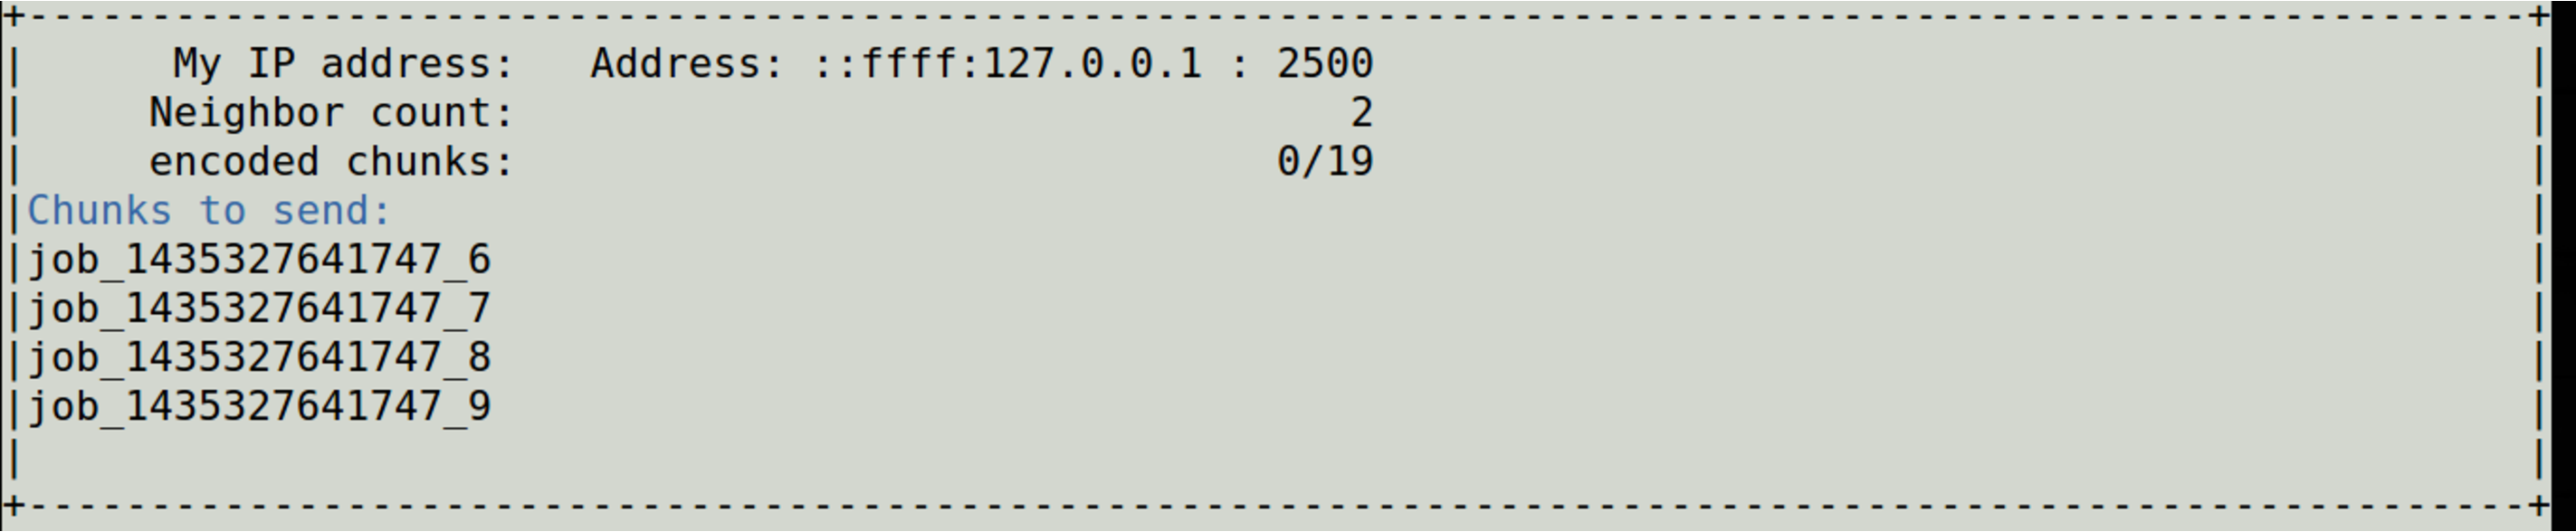
\includegraphics[scale=0.30]{./img/process-initiator.pdf}
\caption{Overview of the process.}
\end{center}
\end{figure}
\begin{figure}[h]
\begin{center}
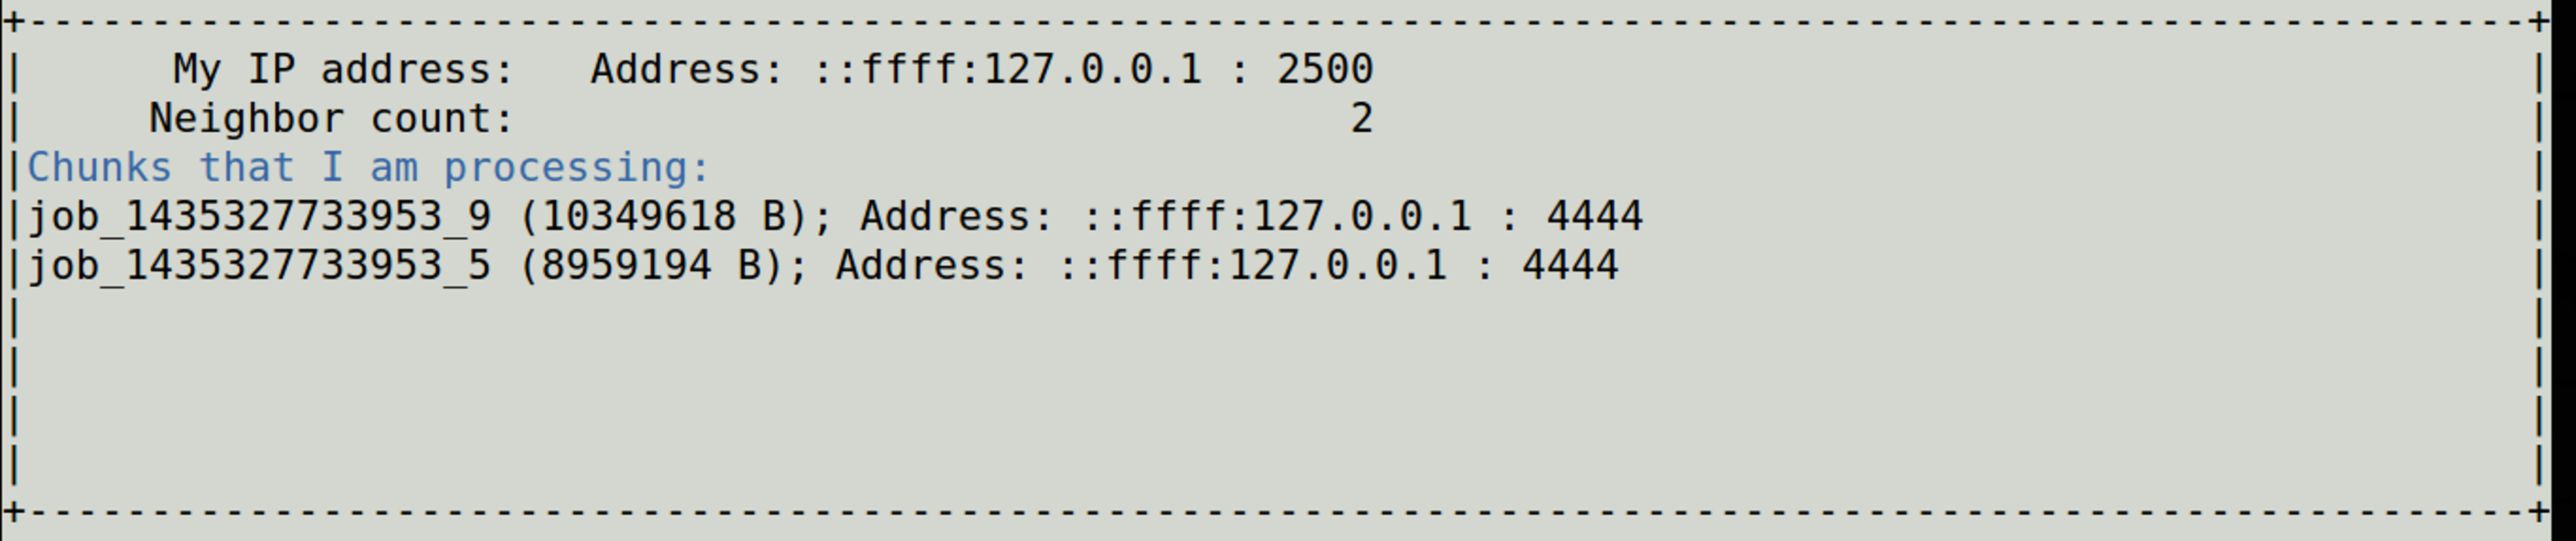
\includegraphics[scale=0.30]{./img/processing.pdf}
\caption{Processing of the tasks.}
\end{center}
\end{figure}
\begin{figure}[h]
\begin{center}
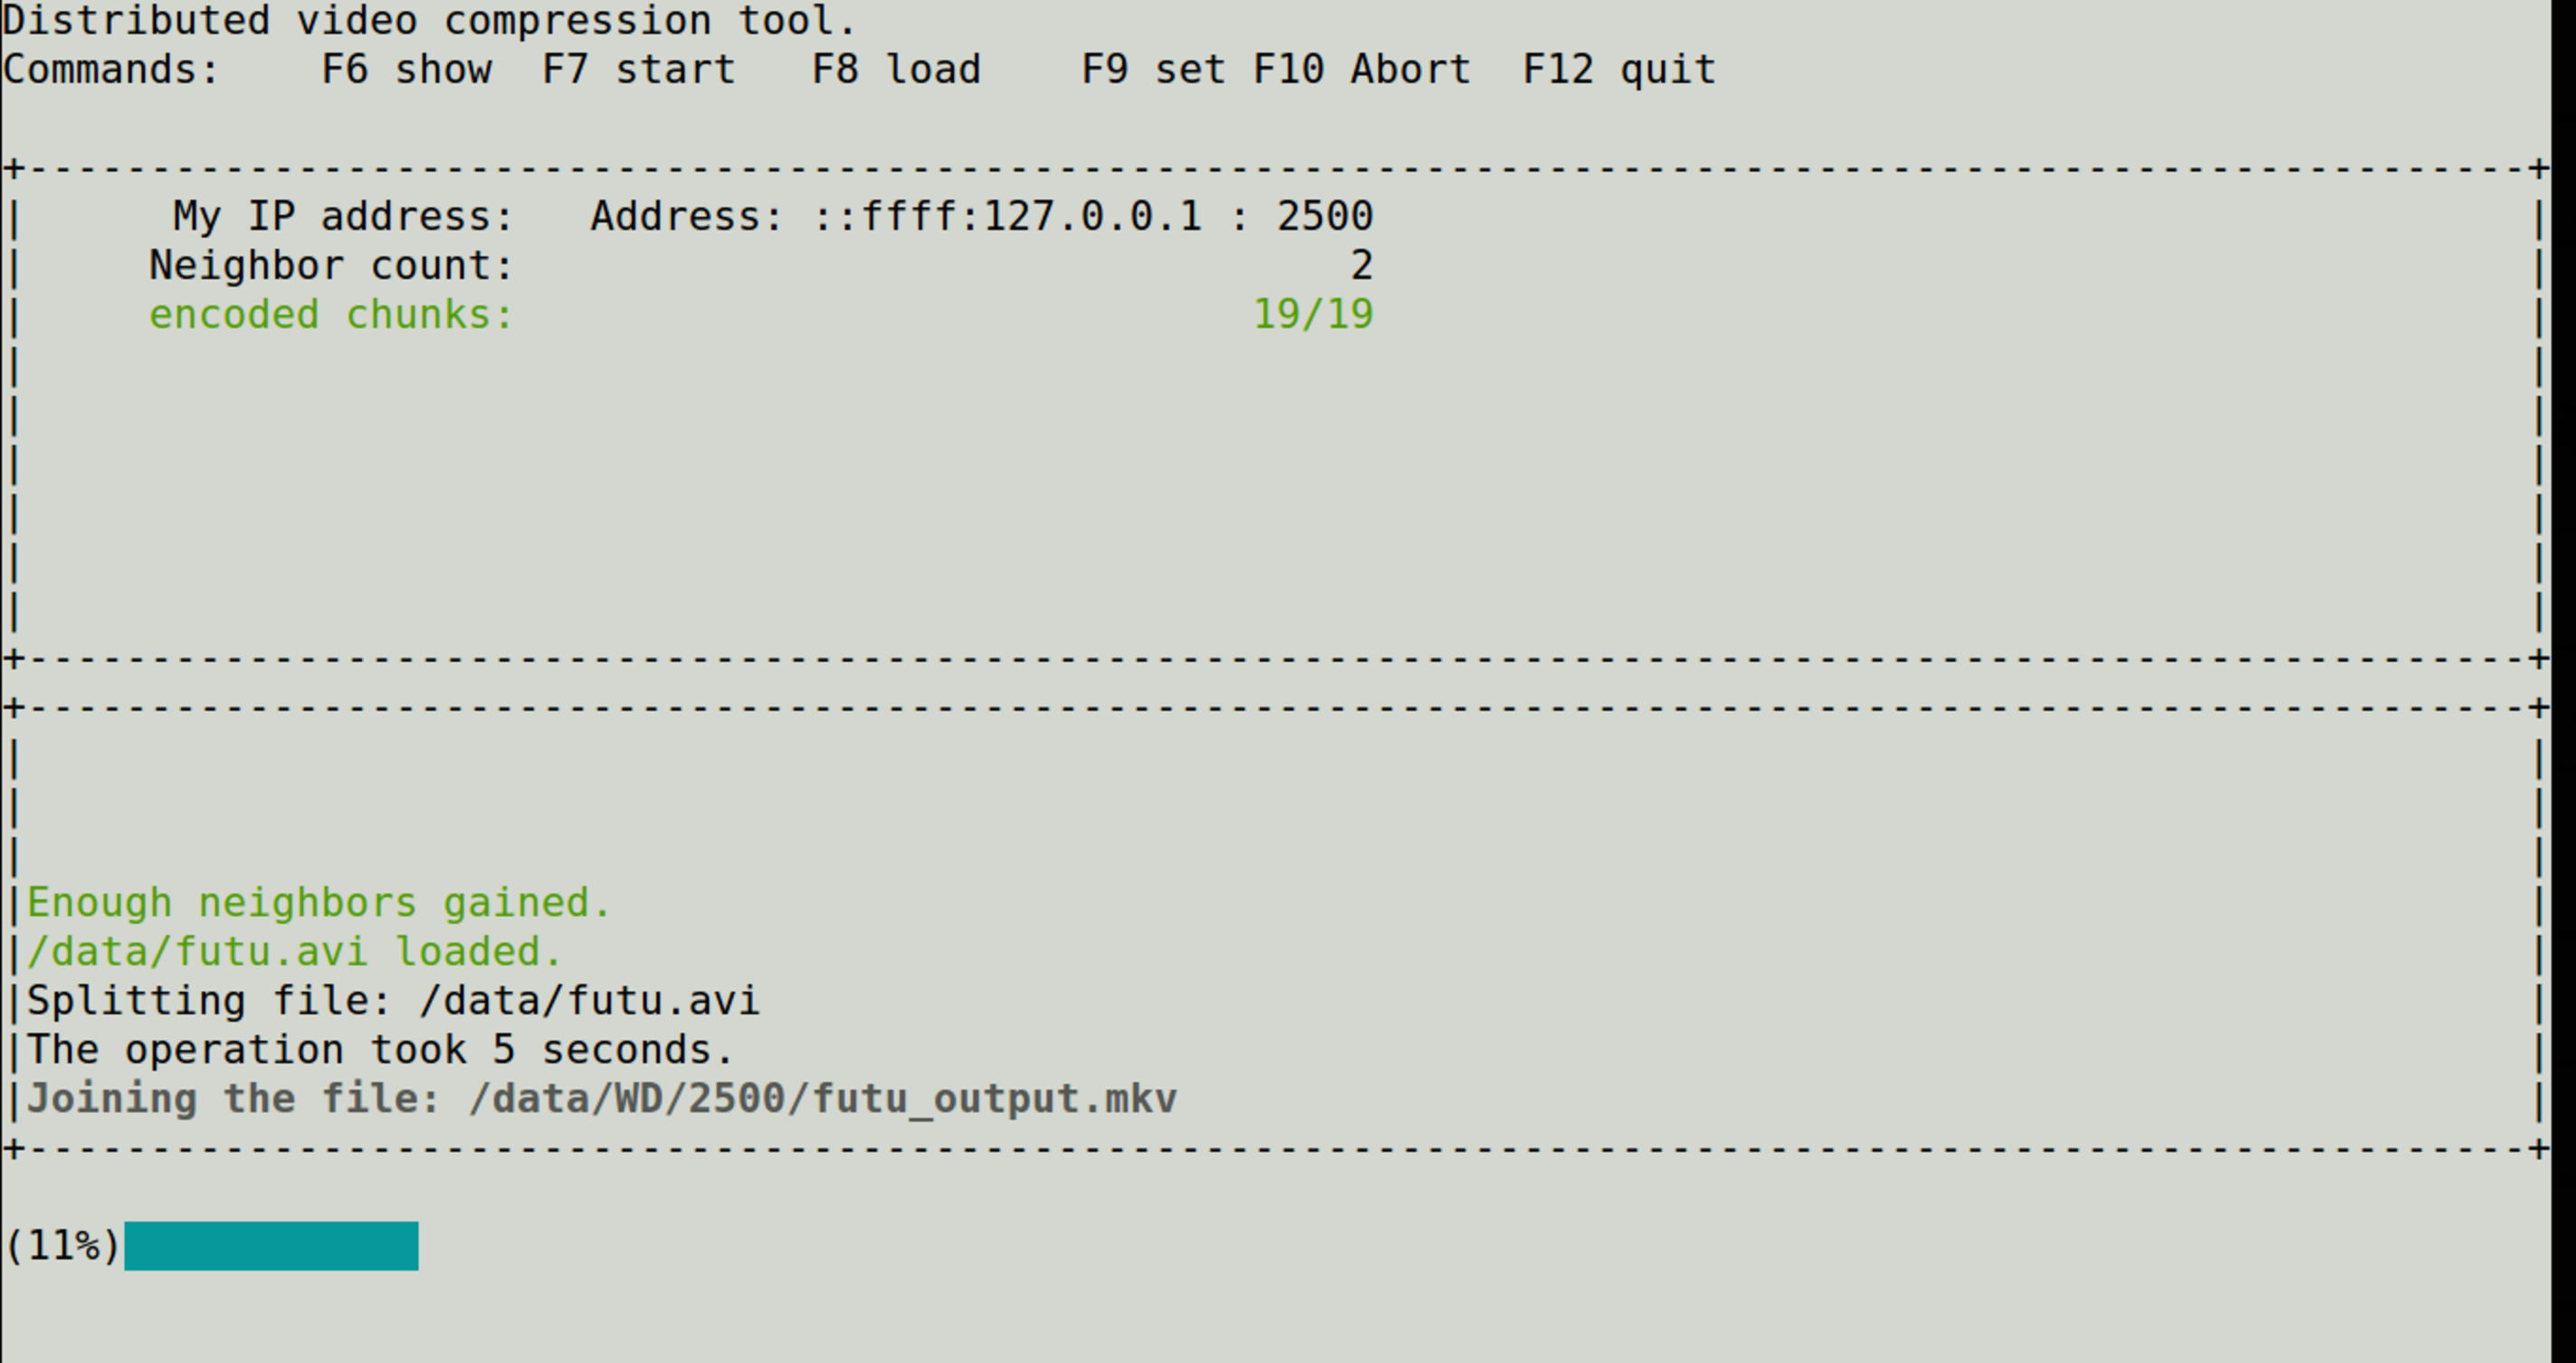
\includegraphics[scale=0.30]{./img/joining.pdf}
\caption{Joining the file.}
\end{center}
\end{figure}

To obtain more information about what is going on, the \textit{-d} option may be used which allows to specify level of debug messages that will be showed.
\section*{Appendix B - Attached software}
All the attached software can be found on the attached CD. It contains:
\begin{enumerate}
\item Sources of the framework, together with the installation script in the \textit{VideoCompression/} directory. This directory also contains the \textit{rapidjson} library and license agreements.
\item Documentation in the \textit{doc/} directory. To view this documentation, it is recommended to open the index.html file in your favorite html browser.
\item FFmpeg and x264 codec sources in the \textit{ffmpeg/} and \textit{x264/} directory.
\end{enumerate} 
\openright\end{document}
